\documentclass[12pt]{extarticle}

\setlength{\headheight}{16pt} % ??? we do what fancyhdr tells us to do  

\title{Advanced Programming and Optimization}
\author{Giacomo Ellero}
\date{a.y. 2024/2025}

\usepackage{preamble}
\usepackage{preamble_svg}
\usepackage{preamble_code}

\renewcommand{\vec}[1]{\bvec{#1}}

\begin{document}

\firstpage

\section{Introduction}

This course will all be about
\begin{align}
	\max f(x), & \text{subject to}                          \\
	g_i(x)     & \leq b_i \quad \text{for } i = 1, \dots, m \\
	x          & \in \R^n
\end{align}
where $f, g_1, \dots, g_m: \R^n \to \R$ are linear functions and $b_1, \dots, b_m \in \R$.
This is the standard \emph{linear programming} problem and can be solved in polynomial time.

However we are also going to be looking at problems where $x \in \Z^n$ (integers).
This is a NP hard problem.

The last part of the course we will have the case where $f, g_1, \dots, g_m$ are not linear
but they are \emph{convex} instead. This also is a hard problem.

\section{Linear programming}

Recall that even though we have stated the problem with less-than-or-equal, we can just multiply
the constraints by $-1$ to flip the inequality if needed.
Similarly we can multiply $f$ by $-1$ to change $\min$ to $\max$ or viceversa.

In linear programming our constraint make a polygon in an $n$-dimensional space.
If we let $\vec a$ be the vector of the coefficients of $f$ the problem reduces to finding the
point which is further away from the origin perpendicular to $\vec a$.

It is not always possible to find an unique solution to a linear programming problem: sometimes
the problem has multiple solutions, it is undecidable, or unbounded.

\subsubsection{Examples}

\begin{example}{Flow}{}
	Recall that the flow problem we saw in CS2 can be written as a linear programming problem:
	each edge has a constraint of $-c_i \leq e_i \leq c_i$ (where $c_i$ is the capacity of each edge)
	and each node has an additional constraint of flow preservation.
	We can maximize the output from the source or the input to the destination.
\end{example}

\begin{example}{Icecream production}{}
	Each month $i$ has a certain icecream demand $d_i$.
	Changing the production of icecream has a cost $a_1$ and the cost of storing icecream we pay $a_2$.
	What is the optimal amount of icecream to be produced?
\end{example}

\begin{proof}[Solution]
	For each month $i$ we want
	\begin{equation}
		x_i + s_{i-1} - s_i = d_i
	\end{equation}
	where $x_i$ is the production of icecream and $s_i$ is the amount we have in storage.

	Our objective will be
	\begin{equation}
		\min a_1 \sum \abs{x_i - x_{i-1}} + a_2 \sum s_i
	\end{equation}
	but this is not a linear function!

	Instead we introduce two new variables $y_i$ which represents the increase in the production
	and $z_i$ which represents the decrease in the production.
	We can now add the constraint
	\begin{align}
		x_i - {x_{i-1}} & = y_i - z_i \\
		y_i             & \geq 0      \\
		z_i             & \geq 0
	\end{align}
	and our objective becomes
	\begin{equation}
		\min a_1 \sum y_i + a_1 \sum z_i + a_2 \sum s_i
	\end{equation}
	which is indeed linear.
	Moreover, we notice that an optimal solution either has $y_i = 0$ or $z_i = 0$,
	hence the problem is equivalent to the first one.
\end{proof}

\subsection{0-sum games}

A 0-sum game has the following properties:
\begin{itemize}
	\item There is a finite set of strategies
	\item Assume player $A$ plays move $i$ and player $B$ plays $j$,
	      then the game pays $m_{ij}$ to player $A$ and $-m_{ij}$ to player $B$.
\end{itemize}
Therefore we can consider the game to be a matrix $M$.

\subsubsection{Example: Colonel Blotto}

\paragraph{Modelling the game}
There are two armies ($B$ and $E$) which are fighting at $3$ mountain passes ($a, b, c$).
$B$ and $E$ have $5$ regiments each.

What each player has to decide is how to partition the regiments:
we will have $k, \ell, m$ such that $k \leq \ell \leq m$ and $k+\ell + m = 5$;
then each group $k, \ell, m$ will be randomly assigned to a mountain pass.

The player who has more regiments in a certain pass will win the pass,
in particular if the number of regiments is the same we will have a draw.
The player who wins more passes wins the game.

We will model the payoff as the probability of winning minus the probability of losing.

\paragraph{Example game 1}
Assume that $B$ plays $i = (0,0,5)$ and $E$ plays $j = (5, 0, 0)$.
Then we have that
\begin{equation}
	m_{ij} = \frac{1}{3} \cdot 0 + \frac{2}{3} \cdot 0 = 0
\end{equation}
where the first probability represents the case where the two armies meet, therefore we have a draw;
the second probability is for all other cases, where one army wins and the other one loses,
therefore we again get a draw.

\paragraph{Example game 2}
Assume that $B$ plays $i = (0,1,4)$ and $E$ plays $j = (5, 0, 0)$.
Then we have that
\begin{equation}
	m_{ij} = \frac{1}{3} \cdot 1 + \frac{2}{3} \cdot 0 = \frac{1}{3}
\end{equation}
similarly to the case above.

\paragraph{How to choose the best strategy}
In this way we can construct a matrix with all the payoffs, however how can we choose the best one?
We could assume that the opponent chooses a strategy at random, therefore we should choose the
strategy with the highest expected payoff, but the enemy is also a skilled player, therefore he
won't choose a strategy at random.

Players will choose based on the worst possible outcome, but then the worst case scenario will
always realize.
Moreover, even if each player knew that the other one is playing the \say{optimal} strategy,
the best option would still be to play the same strategy.
This is called \emph{pure Nash equilibrium}.

\begin{definition}{Pure Nash equilibrium}{pure-nash-eq}
	There exists a pair of pure strategies $(i, j)$ which are the best responses to each other.
\end{definition}

\subsubsection{Rock-Paper-Scissors}

\paragraph{Normal game}
This game does not have a Nash equilibrium, however we can have a mixed strategy.

\begin{definition}{Mixed Nash equilibrium}{mixed-nash-eq}
	$(\tilde x, \tilde y)$ is a mixed Nash equilibrium if each player's response $\alpha(\tilde y)$
	and $\beta(\tilde x)$ is such that
	\begin{equation}
		\beta(\tilde x) = x^T M y = \alpha(\tilde y)
	\end{equation}
\end{definition}

The payoff $(x, y)$ will be
\begin{equation}
	\sum_{i, j} m_{ij} \cdot P(A \text{ plays } i, B \text{ plays } j)
	= \sum_{i, j} m_{ij} x_i y_i = x^T M y
\end{equation}

Therefore in this case, the mixed Nash equilibrium is to choose a strategy uniformly at random:
even if the opponent knew my strategy, there is no better way to respond.

\paragraph{Easter Bunny and Santa Claus}
Assume now that Santa Claus and the Easter Bunny play a game of R-P-S,
however BS doesn't know how to use scissors.

Assume SC chooses strategy $x$, we claim then for each mixed strategy $y$ of the EB,
there exists a pure strategy $y'$ with at least the same payoff.

Indeed EB can achieve
\begin{equation}
	\min \{ \underbrace{x_p - x_s}_{\text{EB plays rock}},
	\underbrace{ -x_r + x_s}_{\text{EB plays paper}}\} = \beta(x)
\end{equation}
Meanwhile SC will max the worst case scenario:
\begin{equation}
	x_0 = \max_{x} \min \{ \underbrace{x_p - x_s}_{\text{EB plays rock}} ,
	\underbrace{ -x_r + x_s}_{\text{EB plays paper}}\}
	= \max_x \beta(x)
	= \max_x \min_y x^T M y
\end{equation}

Therefore SC strategy can be solved through a linear program:
\begin{align}
	\max             x_0 & \quad \text{subject to}                    \\
	x_0                  & \leq x_p - x_s          \label{eq:bunny-r} \\
	x_0                  & \leq -x_r + x_s         \label{eq:bunny-p} \\
	x_p + x_r + x_s      & = 1                                        \\
	x_p, x_r, x_s        & \geq 0
\end{align}
where \cref{eq:bunny-r} is what happens when EB plays rock, \cref{eq:bunny-p} is when EB plays paper
and the other two constraints are there to make sure that $x$ is a valid mixed strategy.
Putting this program into a solver we get that the optimal solution is $\tilde x = (0, 2/3, 1/3)$
and pays $1/3$.

Similarly, for the EB we can write another linear program.
\begin{equation}
	y_0 = \min_{y} \max \{ \underbrace{y_p}_{\text{SC plays rock}} ,
	\underbrace{y_r},
	\underbrace{ -y_r + y_p}_{\text{EB plays paper}}\}
	= \min_x \alpha(x)
	= \min_x \max_y x^T M y
\end{equation}
Hence
\begin{align}
	\min y_0  & \quad \text{subject to} \\
	y_0       & \leq y_p                \\
	y_0       & \leq y_r                \\
	y_0       & \leq -y_r + y_p         \\
	y_p + y_r & = 1                     \\
	y_p, y_r  & \geq 0
\end{align}
and solving the program gives that the optimal solution is $\tilde y = (1/3, 2/3)$ which pays $1/3$
(therefore EB loses).
Note that this is the same win that SC gets.
We have
\begin{equation}
	\tilde x_0 = \beta(\tilde x) \leq \tilde x^T M \tilde y \leq \alpha(\tilde y) = \tilde y_0
\end{equation}
therefore $(\tilde x, \tilde y)$ is a mixed Nash equilibrium.

\begin{theorem}{Von Neumann}{vn}
	In a finite zero-sum game $x_0 = y_0$.
	Therefore it does not matter who chooses the strategy first.
\end{theorem}


\subsubsection{AA}

We want to find a line $y = ax + b$ which separates two kind of points $p$ and $q$
such that $p$ are above the line and $q$ are below.
We try to write this as a linear problem
\begin{align}
	y(p_i) > ax(p_i) + b \quad \forall i = 1, \dots, m \\
	y(q_i) < ax(q_i) + b \quad \forall i = 1, \dots, m
\end{align}

However, this is not a linear program, because the inequality are strict.
We can fix this by introducing another variable $\delta$ and a constraint $\delta \geq 0$,
moreover we also need to $\max$ is, since, ideally we'd like for $\delta$ to be $> 0$ but, again,
we are not allowed to have strict inequalities.
\begin{align}
	\max \delta & \text{ subject to}                                   \\
	y(p_i)      & > ax(p_i) + b + \delta \quad \forall i = 1, \dots, m \\
	y(q_i)      & < ax(q_i) + b + \delta \quad \forall i = 1, \dots, m \\
	\delta      & \geq 0
\end{align}

\subsection{Affine and convex geometry}
\subsubsection{Affinity}

Let $L$ be a linear subspace of $\R^d$.
Then $A = a + L$ with $a \in \R$ is a shifted linear subspace: we call it an \emph{affine space}.

Firstly we note that $A = a + L = x + L$ $\forall x \in A$: indeed if $x \in A$ then $x-a \in L$,
then for $y \in a + L$ we have that $y - a - (x - a) \in L$ giving $y \in x + L$.

We also define the \emph{affine hull} of $X \subseteq \R^d$ to be the intersection of all affine
subspaces containing $X$.

\begin{proposition}{}{}
	The affine hull of $X \subseteq \R^d$ can be written as
	\begin{equation}
		\mathrm{aff. hull}(X) =
		\left\{ \sum \alpha_i x_i \left| \substack{x_i \in X \\ \sum \alpha_i = 1} \right. \right \}
	\end{equation}
\end{proposition}
\begin{proof}
	First we prove that the set of affine combinations is included in the affine hull.
	By definition of affine hull we have $X \subseteq A = x_1 + L$.
	Moreover
	\begin{equation}
		\sum x_i \alpha_i = x_1 + \left(\sum \alpha_i (x_i - x_1)\right) \in x_1 + L = A
	\end{equation}

	Then we prove that affine hull is included in the set of affine combinations.
\end{proof}

Now we consider the dimensions of these spaces:
\begin{itemize}
	\item $\dim(L) =$ max number of linear independent vectors in $L$.
	\item $\dim(A) = \dim(L)$.
	\item $\dim(X) = \dim(\mathrm{aff. hull}(X))$.
	\item $\dim(\varnothing) = -1$
\end{itemize}
take these as definitions.

In particular a point is an affine space with dimension 0, a line has dimension 1,
a plane has dimension 2, and an hyperplane in $\R^d$ has dimension $d-1$.
Moreover, note that hyperplanes can be written as
\begin{equation}
	\{ x: \R^d \mid a^T x = b \}
\end{equation}

Observe that affine spaces spaces $A$ of dimensions $k \leq d-1$ are intersections of hyperplanes
(proof in lecture notes).

We call \emph{halfspace} the set
\begin{equation}
	\{x \in \R ^d : a^T x \leq b \}
\end{equation}

\subsubsection{Convexity}

We define the convex hull of a set $X$ as the intersection of all convex sets containing $X$.
Moreover we define a convex combination as $\sum \alpha_i x_i$ such that $x_i \in X$ and
$\sum \alpha_i = 1$.

The convex hull of $X$, i.e. $\conv(X)$ has the following properties:
\begin{itemize}
	\item $\conv(X)$ is convex itself
	\item $\conv(X)$ is the set of convex combinations of elements of $X$, that is
	      \begin{equation}
		      \conv(X) =
		      \left\{ \left.\sum_{i = 1}^k \alpha_i x_i \,\right|\, k \in \N^+ , x_i \in X, \sum_{i = 1}^k \alpha_i = 1 \right\}
	      \end{equation}
	\item $\conv(X) \subseteq X$
	\item For $X$ finite $\conv(X)$ is compact (closed and bounded)
\end{itemize}

\begin{theorem}{Caratheodory}{caratheodory}
	Let $X \subseteq \R^n$ and $d = \dim X$.
	Then
	\begin{equation}
		\conv(X) =
		\left\{ \left.\sum_{i = 1}^{d+1} \alpha_i x_i \,\right|\, x_i \in X, \sum_{i = 1}^k \alpha_i = 1 \right\}
	\end{equation}
\end{theorem}

\begin{proof}
	We know that there exists $k \in \N^+$ such that the theorem is true, let $k$ be the smallest one.
	If $k \leq d + 1$ we are done as we can set the remaining coefficients to $0$.

	We will show by contradiction that it is not possible that $k > d + 1$.
	Let $\{x_1, \dots, x_k\} = X'$: they are affine dependant;
	then there exists $\beta \neq 0 \in \R^k$ s.t. $\sum \beta_i x_i = 0$ and $\sum \beta_i = 0$.

	We know that for any $x \in X$ we can find $\alpha_i$ such that $x = \sum^k_{i = 1} \alpha_i x_i$.
	Let $\gamma = \max\{\frac{\alpha_i}{\beta_i} \mid i = 1, \dots, k_i, \beta_i < 0\}$
	and $\alpha_i' = \alpha_i - \gamma \beta_i$, such that $\alpha_i \geq 0$ and there exists exactly
	one $i^*$ such that $\alpha_{i^*}' = 0$.

	Note that
	\begin{equation}
		\sum \alpha_i' = \underbrace{\sum \alpha_i}_{=1} + \underbrace{\sum \gamma \beta_i}_{= 0} = 1
	\end{equation}
	But then $\sum \alpha_i' x_i = x$ since $\sum \beta_i x_i = 0$ and by our choice of $\alpha_i'$
	we know that $\alpha_{i^*}' = 0$ therefore we can remove the $i^*$-th term of the combination
	without changing the result.
	In this way we decreased $k$ by $1$.
	We can continue iteratively until $k = d+1$.
\end{proof}

\begin{theorem}{Strong convex separation}{strong-conv-sep}
	Let $C, D \subseteq \R^d$ be non-empty, convex, closed, and disjoint,
	moreover $C$ is bounded and therefore compact.
	Then, there is a hyperplane $\{x \mid a^T x = b\}$ such that
	$C \subseteq \{ \mid a^T x < b\}$ and $D \subseteq \{ x \mid a^T x > b\}$.
\end{theorem}

\begin{proof}
	Find $c \in C, d \in D$ such that $\norm{c-d}$ is minimal.
	Note that we can do this only if $C$ and $D$ are compact.
	If $D$ is also compact we are done.

	If $D$ is unbounded we choose $c'\in C, d' \in D$ and $\beta = \norm{c' - d'}$,
	$\alpha = \mathrm{diam}(C)$ (the diameter of $C$).
	Then consider the ball $B$ defined as $B = \{x \mid \norm{c' - x} \leq \alpha+\beta\}$.
	The set $D'= D \cap B$ is now compact and for $x \in C$ and $y \in D$, if $\norm{x - y} \leq \beta$,
	$y \in D'$:
	\begin{equation}
		\norm{c'-y} \leq \norm{c' - x} + \norm{x - y} \leq \alpha + \beta
	\end{equation}
	Now we choose $(c, d) = \argmin_{c \in C, d \in D'} \{\norm{c - d}\}$.

	We now choose an hyperplane using the parameters $a, b$:
	\begin{equation}
		a \coloneq d - c \quad \text{and} \quad b \coloneq \frac{a^T d - a^T c}{2}
	\end{equation}
	then
	\begin{equation}
		a^Td - a^T c = a^T a = \norm{a}^2 = \norm{d - c}^2 \geq 0
		\implies a^T d > a^T c
	\end{equation}

	Now we want to prove that $\forall x \in C: a^Tx < b$ and $\forall y \in D: a^T y > b$.
	We show that $a^T x \leq a^T c < b$ and we can do the same procedure over $D$.

	By contradiction assume that $a^Tx > a^Tc$.
	We have $a^T(x-c)>0$ which means that the angle $d, c, x$ is sharp (acuto) and we can draw
	a right-angle triangle we can form with $x' \in \conv(\{c, x\})$ and
	$\norm{x'-d}<\norm{c-d}$, but this contradicts the fact that $c$ is minimal.
\end{proof}


\begin{theorem}{Weak convex separation}{weak-conv-sep}
	Let $C, D$ be convex and disjoint.
	Then there is an hyper plane $\{x \mid a^T x= b\}$ such that
	$C \subseteq \{ \mid a^T x \leq b\}$ and $D \subseteq \{ x \mid a^T x \geq b\}$.
\end{theorem}

\begin{proof}
	Consider $\{0\}$ and $S = \{x - y \mid x \in C, y \in D\}$.
	Let $x - y \in S$ and $x' - y' \in S$, then take their convex combination:
	\begin{equation}
		t(x - y) + (1-t)(x'-y') =
		\underbrace{tx + (1-t)x'}_{\in C} - \underbrace{(ty + (1-t)y')}_{\in D} \in S
	\end{equation}
	Now we have a few possible cases:
	\begin{enumerate}
		\item $0 \notin \mathrm{cl}(S)$ ($0$ is in the closure of $S$).

		      We apply \cref{thm:strong-conv-sep} to $\{0\}$ and $\mathrm{cl}(S)$.
		      We have
		      \begin{equation}
			      0 = a^T 0 < b , a^T(x-y) \enspace \forall x-y \in S
			      \implies a^T x > a^T y \enspace \forall x \in C, d \in D
		      \end{equation}

		\item $0 \in \mathrm{cl}(S)$.

		      Then $0$ is in the boundary of $\mathrm{cl}(S)$.
		      \begin{enumerate}
			      \item If $\mathrm{int}(S) = \varnothing$, then $S$ belongs to a hyperplane
			            $\{x \mid a^T = 0 \}$ which we can use as separator: we have
			            $a^T x =  a^T y$ for all $x \in C, y \in D$.

			      \item If $\mathrm{int}(S) \neq \varnothing$ we define
			            $S_{-\varepsilon} = \{s \in S \mid B_\varepsilon(s) \subseteq S\}$
			            for some $\varepsilon > 0$.
			            Then $\mathrm{cl}(S_{-\varepsilon})$ is closed, convex and does not contain $0$,
			            therefore we can apply \cref{thm:strong-conv-sep}
			            and get some $a_\varepsilon, b_\varepsilon$ such that
			            $a_\varepsilon^T s > 0$ for all $s \in S_{-\varepsilon}$.

			            Now we normalize $a_\varepsilon$ such that $\norm{a_\varepsilon} = 1$
			            and choose an infinite sequence $\varepsilon_n$
			            which converges to $0$ as $n\to\infty$.
			            Since is bounded ($\norm{a_{\varepsilon_k}} = 1$) the sequence $a_{\varepsilon_n}$
			            contains a subsequence converging to $a\neq 0$.

			            Since $a_{\varepsilon_k}^T s > 0$ for all $s \in S$ and for all $k$, we have
			            $a^T s > 0$ for all $s \in \mathrm{int}$ and $a^T s \geq 0$ for all $s \in S$.
		      \end{enumerate}
	\end{enumerate}
	Therefore we have proven that $a^Ts \geq 0 \implies a^T(x-y) \geq 0$ which gives the result of
	$a^T x \geq a^T y$.
\end{proof}

\subsection{Duality}

\begin{definition}{Standard form}{lp-standard}
	Given $A \in \R^{m\cross n}, b \in \R^m, c \in \R^n$
	a linear program where the variables are $n$ dimensional and there are $m$ constraints
	can be written as
	\begin{align}
		\max c^T x & \text{ subject to} \\
		Ax \leq    & b                  \\
		x \in \R^n
	\end{align}
\end{definition}

Moreover any LP can be written in this form by adding another constraint when we have equalities,
flipping the signs of $\geq$ and of the objective function if needed.
We note that this is equivalent to finding an intersection between halpspaces, and when we require
$Ax = b$ we are instead finding an intersection between hyperplanes.

We now want to find a bound for the objective function, that is $h$ such that $c^T x \leq h$.
To do so we look for a vector $d$ such that $d_i \geq c_i$ and $h$ as small as possible.
To find such $d$ we take the constraints of the original problem and
take linear combinations of them: let $y$ be a vector in $\R^m$
(where $m$ is the number of contraints we have) and we take $y_i$ times the $i$-th constraint;
then $d_i = \sum_{j} A_{ji} y_j$.

\begin{definition}{Dual of a LP}{dual}
	In general, for a given LP in standard form (\cref{def:lp-standard}) called primal
	we can write its \emph{dual} (where $A, c, b$ are the same as primal):
	\begin{align}
		\min b^T x & \text{ subject to} \\
		A^T y =    & c                  \\
		y \geq 0
	\end{align}
\end{definition}

\subsubsection{Weak duality}

\begin{theorem}{Weak duality}{weak-duality}
	Given an LP (P) and its dual (D), for each $x$ feasible to (P) and each $y$ feasible to (D)
	we have $c^T x \leq b^T y$.
\end{theorem}

\begin{proof}
	We have
	\begin{equation}
		c^T x = (A^T y)^T x = y^T A x \leq y^T b
	\end{equation}
	where the first equality is due to $A^T y = c$ (\cref{def:dual}) and the last
	inequality is because $Ax \leq b$ and $y \geq 0$.
\end{proof}

\begin{corollary}{}{}
	If (P) is unbounded then (D) in infeasible and viceversa.
\end{corollary}

\subsubsection{Farkas lemma}

\begin{definition}{Convex cone}{convex-cone}
	A set $C \subseteq \R^n$ is a convex cone if for all $x, y \in C$ and $\lambda, \mu \in \R^+$
	we have $\mu x + \lambda y \in C$.
\end{definition}

We call $\mathrm{cone}(X)$ the smallest cone containing $X$.

We now state some facts about convex cones without proof.

\begin{proposition}{Facts about convex cones}{facts-cones}
	The following facts are true for any convex cone:
	\begin{enumerate}[label=\roman*.]
		\item Every cone contains $0$;
		\item The smallest cone containing $X$ is
		      \begin{equation}
			      \mathrm{cone}(X) =
			      \left\{ \sum^k_{i = 1} \lambda_i x_i \mid k \in N^+, x_i \in X, \lambda_i \geq 0 \right\}
		      \end{equation}
		\item If $\abs{X}$ is finite then $\mathrm{cone}(X)$ is closed.
	\end{enumerate}
\end{proposition}

\begin{figure}[h!]
	\centering
	\includesvg[width=0.3\textwidth]{./assets/advanced-programming/convex-cone.svg}
	\caption{Two convex cones: the red one consists of all points such that $\mu x + \lambda y$.
		The curves on the top-right edge represent the region continues infinitely.}
\end{figure}

\begin{theorem}{Farkas lemma}{farkas}
	Let $a_1, \dots, a_n, b \in \R^m$ and $A = \{a_1, \dots, a_n\} \subset \R^m$.
	Then exactly one of the following cases occurs:
	\begin{enumerate}[label=\roman*.]
		\item $b \in \mathrm{cone}(A)$;
		\item There is a hyperplane passing through $0$ of the form $h = \{x \in \R^m \mid y^Tx = 0\}$
		      such that $\mathrm{cone}(A)$ is on one side of the cone
		      (i.e. $y^T a_i \geq 0$ for all $i = 1, \dots, n$) and $b$ lies on the other side
		      (i.e $y^T b < 0$).
	\end{enumerate}
\end{theorem}

\begin{proof}
	First note that i. and ii. cannot hold at the same time, since i. implies that $y^T b \geq 0$
	but ii. implies the opposite, therefore we just need to prove that
	if i. is false then ii. is true.

	Let $C = \mathrm{cone}(A)$ and assume that $b \notin C$.
	Let $D = \{b\}$ then $D$ is compact, $C$ is closed by \cref{prop:facts-cones} and they are both
	convex, therefore we can apply \cref{thm:strong-conv-sep} to find a hyperplane
	$h' = \{ x \in \R^m \mid y^T x = \gamma\}$ such that $y^T b < \gamma$ and $y^T c > \gamma$
	for all $c \in C$. Note that since $0 \in C$ we have that $\gamma < 0$.

	Now choose $h = \{ x \in \R^m \mid y^T x = 0\}$, then $0 \in h$, $y^T b < \gamma < 0$
	therefore $b$ is on one side of $h$.
	Now we want to prove that $y^Tc \geq 0$ for all $c \in C$ so that $h$ is the hyperplane we are
	looking for.

	Assume, by contradiction, that $y^T c < 0$ for some $c \in C$.
	Then $\frac{2 \gamma}{y^T c} c \in C$ since $\frac{2 \gamma}{y^T c} \geq 0$ and
	$C$ is a convex cone.
	But then $y^T \frac{2 \gamma}{y^T c} c = 2 \gamma < \gamma$ which is a contradiction.
\end{proof}

\begin{corollary}{Farkas lemma in matrix form}{farkas-matrix}
	Let $A \in \R^{m \cross n}$ and $b \in \R^m$.
	Then exactly one of the following holds:
	\begin{enumerate}[label=\roman*.]
		\item There is $x \in \R^n$ such that $Ax = b$ and $x \geq 0$.
		\item There is $y \in \R^m$ such that $y^T A \geq 0^T$ and $y^T b < 0$.
	\end{enumerate}
\end{corollary}

\begin{proof}
	Let $a_1, \dots, a_n \in \R^m$ the columns of $A$, then $x$ defines a non-negative combination of
	$a_1, \dots, a_n$ so that $b$ is in their cone, and $y$ defines the hyperplane $h$.
\end{proof}

\subsubsection{Strong duality}

\begin{lemma}{}{strong-duality-claim}
	Let $x\in \R^n$ be such that $Ax \leq b$, then the following statements are equivalent:
	\begin{enumerate}[label=\roman*.]
		\item For all $x\in \R^n$ such that $Ax \leq b$ there holds $c^T x \leq \delta$.
		\item There is $y \in \R^m$ such that $y \geq 0$, $A^T y = c$, and $b^T y \leq \delta$.
	\end{enumerate}
\end{lemma}

This lemma tells us that for every valid upper bound $\delta$ of the objective of (P) there is a
solution $y$ of (D) which certifies it.

\begin{proof}
	We prove the two directions separately.
	\begin{description}[font=\normalfont\itshape]
		\item[i. $\implies$ ii.]
		      By weak duality we have
		      \begin{equation}
			      c^T x = (y^T A)x \leq y^T b \leq \delta
		      \end{equation}
		\item[ii. $\implies$ i.] We will show that if ii. is false then there is no $x$ such that
		      $Ax \leq b$ and $c^T > \delta$.

		      Assume that there is no $y \in \R^m$ and no $\lambda \in \R$ with $y, \lambda \geq 0$
		      such that
		      \begin{align}
			      A^Ty         & = c      \\
			      b^Ty+\lambda & = \delta
		      \end{align}

		      TODO
		      \qedhere
	\end{description}
\end{proof}

\begin{theorem}{Strong duality}{strong-duality}
	Given a LP (P) and its dual (D) (as in \cref{def:lp-standard} and \cref{def:dual})
	exactly one of the following cases occurs:
	\begin{enumerate}[label=\roman*.]
		\item Both (P) and (D) are infeasible;
		\item (P) is unbounded and (D) is infeasible;
		\item (D) is unbounded and (P) is infeasible;
		\item Both (P) and (D) have a feasible solution, then the optimal solutions $x^*$ of (P)
		      and $y^*$ of (D) both exists and are such that $c^T x = b^T y$.
	\end{enumerate}
\end{theorem}

\begin{proof}
	Cases i., ii., and iii. are already covered by weak duality, we are left to prove iv.

	Assume that (P) has a feasible solution, and let
	$\delta = \sup_{x \in \R^b} \{c^T x \mid Ax \leq b\}$ be the objective for $x$ optimal.
	Note that $-\infty < \delta < \infty$ since this solution exists and (P) is bounded.

	By weak duality we have that $\delta \leq b^T y$ for each $y$ feasible to (D)
	and by \cref{lemma:strong-duality-claim}, we find $y \geq 0$ such that $A^T y = c$ and
	$b^T y \leq \delta$, then $\delta \leq b^T y \leq \delta \implies b^T y = \delta$ and $y$ is an
	optimal solution to $(D)$.
\end{proof}

\begin{theorem}{Complementary slackness conditions}{complementary-slackness}
	Let $x$ be a feasible solution to (P) and $y$ a feasible solution to (D).
	Then $x,y$ are optimal if and only if $y^T(b-Ax) = 0$.
\end{theorem}

\begin{proof}
	By \cref{thm:strong-duality} if $x, y$ are optimal we have $c^T x = b^T y$.
	Then
	\begin{equation}
		0 = y^T b - c^T x = y^T b - (A^T y)^T x = y^T (b - Ax)
	\end{equation}
	as desired.
\end{proof}

Note that since $y \geq 0$ and $b - Ax \geq 0$, for each $i$, if $y_i > 0$ then $b_i-a_i^T x = 0$
(the $i$-th constraint is tight) or if $b_i-a_i^T x > 0$ then $y_i = 0$.


\section{Simplex method}

\subsection{Geometry of polyhedra}

\begin{definition}{Polyhedron and polytope}{polyhedron-polytope}
	\begin{itemize}
		\item A polyhedron is an intersection of a finite number of halfspaces;
		\item A polytope is a bounded polyhedron.
	\end{itemize}
\end{definition}

There are some notable types of polyhedra:
\begin{description}
	\item[Cubes] They are polytopes with $2n$ constraints in $[-1, 1]^n$ defined as
	      $\{x \mid \norm{x}_\infty \leq 1\}$, or equivalently we have
	      \begin{align}
		      x_i & \leq 1  & \text{for all } i = 1, \dots, n \\
		      x_i & \geq -1 & \text{for all } i = 1, \dots, n
	      \end{align}
	      Cubes have $2n$ constraints and $2^n$ vertices.

	\item[Cross polytope] These are polytops defined as $\{ x \in \R^n \mid \norm{x}_1 \leq 1\}$
	      where $\norm{x}_1 = \sum \abs{x_i} \leq 1$.
	      To write it in constraint form we write:
	      \begin{equation}
		      \forall \sigma \in \{\pm 1\}^n : \sigma^T x \leq 1
	      \end{equation}
	      which is equivalent to the definition above.
	      Cross polytopes have $2^n$ constraints and $2n$ vertices.

	\item[Simplex] An $n$ dimensional simplex has $n + 1$ vertices and is better defined in
	      $n+1$ dimensions.
	      \begin{equation}
		      x_i \geq 0 \quad \forall i = 1, \dots, n+1 \quad \text{s.t. } \sum x_i = 1
	      \end{equation}
\end{description}

\begin{definition}{Face}{face}
	A face of a polyhedron $P$ is a subset $F \subseteq P$ such that there exists a non-zero vector
	$c \in R^n$ and a number $z \in R$ such that $c^T x = z$ for all $x \in F$ and $c^T x < z$
	for all $x \in P \setminus F$.

	In other words there exists an hyperplane that touches $P$ exactly at $F$.

	Note that also $P$ itself and $\varnothing$ fall into this definition.
	To differentiate them, we say that the other faces $F \neq P$ and $F \neq \varnothing$ are
	\emph{proper faces}.
\end{definition}

\begin{theorem}{Minkowski-Weyl for polytopes}{minkowski-weyl-polytopes}
	$P \subseteq \R^n$ is a polytope if and only if $\exists V \subseteq \R^n$ finite such that
	$P = \conv(V)$ (convex hull of $V$).
\end{theorem}

\begin{theorem}{Minkowski-Weyl for polyhedra}{minkowski-weyl-polyhedra}
	$P \subseteq \R^n$ is a polytope if and only if $\exists V, Y \subseteq \R^n$ finite such that
	$P = \conv(V) + \mathrm{cone}(Y)$ (convex hull of $V$ plus
	the convex cone of $Y$ (as in \cref{def:convex-cone}),
	the sum is defined as $A + B = \{ x+ y \mid x \in A, y \in B$).
\end{theorem}

Therefore, as a consequence of these theorems we have two ways of writing each polytope:
$P = \{x \mid A x \leq b\} = \conv(V)$.
There formulation are equivalent from the meaning point of view, but they are very different from
the computational point of view: we saw how cross polytopes have $2^n$ constraints but just $2n$
vertices.
We can prove that the optimal solution of an optimization problem is on a vertex, however this
is often not good enough as we could need to check $2^\abs{V}$ vertices, which are too many.

Let $P$ be a polyhedra defined as $P = \{x \mid A x \leq b\}$. Then, note that if we choose some
$i$ and we make the inequality strict, that is $A_i x = b$ we get a face.
Moreover, if we do this procedure for some $i$ \emph{and} $j$ we obtain a vertex.
This result is formalized in the following lemma.

\begin{lemma}{Equivalent definitions of faces}{faces}
	The following definitions of faces are equivalent:
	\begin{enumerate}
		\item \Cref{def:face}:
		      \begin{equation}
			      F = P \cap \{ x \mid c^T x = \delta \} \quad \text{s.t. }
			      \substack{c \neq 0 \\ c^T x \leq \delta \enspace \forall x \in P_i}
		      \end{equation}
		      Moreover, $F = \varnothing$ and $F = P$ are also valid faces.
		\item $F = \{ x \in P \mid A'x = b'\}$ for some subsystem $A'x \leq b'$ of
		      $Ax \leq b$.
	\end{enumerate}
\end{lemma}

\begin{proof}
	We prove each direction separately.
	\begin{description}[font=\normalfont\itshape]
		\item[(1) $\implies$ (2)]
		      We can rewrite $F$ as $F = \{ x \in P \mid c^T = \delta\}$ and
		      $\delta = \max \{ c^T x \mid x \in P\}$.
		      This is a linear program, therefore we can use \cref{thm:strong-duality} and write
		      $F = \min \{b^T y \mid A^T y = c, y \geq 0 \}$.

		      By complementary slackness (cf. \cref{thm:complementary-slackness}),
		      we have that if $x, y$ are feasible $y^T(Ax - b) = 0$ and
		      $y_i \geq 0$ implies $(Ax - b)_i = 0$ and $(Ax - b)_i < 0$ implies that $y_i - 0$,
		      so that by knowing the solution to the dual we can check which constraints are tight
		      in the primal.

		      Then for all $x \in P$ we have that $c^T x = \delta$ iff $x$ is optimal, which in turns
		      holds iff $(y^*)^T(b - Ax) = 0$ by complementary slackness, which again is equivalent
		      to $Ax'= b'$.

		\item[(2) $\implies$ (1)]
		      If $F = \{ x \in P \mid A'x = b'\} \neq \varnothing$ then $c$ is the sum of the rows
		      of $A'$ and $\delta$ is the sum of the entries in $b'$.
		      Then, for each $x \in P$ we have that $A'x\leq b'$ and $c^T x = \delta$ if and only if
		      $A'_i x = b_i'$ for all $i$ implying $F = \{ x \in P \mid c^T x = \delta \}$.
		      \qedhere
	\end{description}
\end{proof}

First we note that $P$ has a finite number of faces.
Moreover, if $E \subseteq F$ and $E$ is a face of $F$, then $E$ is a face of $P$.

We can define a polyhedron in an even more generic way, that is
\begin{equation}
	P = \{ x \in \R^n \mid \underbrace{A'x = b'}_{m' \text{ number of equalities}},
	\underbrace{A '' x \leq b''}_{m'' \text{ number of inequalities}} \}
	\label{eq:poly-desc}
\end{equation}
Using this description we can define the minimal description of $P$.
\begin{definition}{Minimal description of a polyhedron}{poly-minimal-desc}
	Let $P$ as in \cref{eq:poly-desc}.
	That is a minimal description if
	\begin{itemize}
		\item All rows of $A'$ are linearly independent;
		\item Omitting any of the inequalities changes the polyhedron;
		\item Converting an inequality to	an equality also changes the polyhedron.
	\end{itemize}
\end{definition}

We note that if we consider a minimal description of $P$ and $P \neq \varnothing$,
then there exists $z \in P$ such that $A''z < b$ (see lecture notes for proof, lecture 10).

\begin{lemma}{Dimension of proper faces}{dim-faces}
	If there exists $z \in P \neq \varnothing$ such that $A'' z<b''$, then
	\begin{itemize}
		\item $\mathrm{dim}(P) = n - \rank(A')$;
		\item $z$ does not belong to any proper face of $P$.
	\end{itemize}
\end{lemma}

\begin{proof}
	Let $A = \{ x \mid A'x = b\}$, since $P \subseteq A$ we have
	$\dim(P) \leq \dim(A) = n - \rank(A)$.
	Then, since the inequality is strict, we can find $\varepsilon > 0$ such that the ball
	$B = \{ x \in A \mid \norm{x - z} \leq \varepsilon \} \subseteq P$ which in turns implies
	$\dim(P) \geq \dim(B) = \dim(A)$.

	To prove the second part we consider any $h = \{x \mid a^T x = b\}$ such that $a^T z = b$
	and $A \subseteq h$.

	TODO: lecture 11
\end{proof}

\begin{corollary}{}{}
	Let $F$ be a proper face of $P$, then $\dim(F) \leq \dim(P) -1$.
\end{corollary}

\begin{proof}
	Consider a minimal description of $P$.
	Then $F$ can be written as
	\begin{equation}
		F = \{ x \in \R^n \mid A'x = b', \tilde A x = \tilde b, A'' x \leq b'' \}
	\end{equation}
	where $\tilde A x \leq \tilde b$ is a subsystem of $A '' x \leq b ''$.
	Then $\dim(F) \leq n - \rank\begin{pmatrix} A' \\ \tilde A \end{pmatrix}$.

	If $\rank\begin{pmatrix} A' \\ \tilde A \end{pmatrix} = \rank(A')$ then
	either each inequality of $\tilde A x = \tilde b$ is a linear combination of $A' x = b'$
	and $F = P$, otherwise we have
	\begin{equation}
		\rank \begin{pmatrix} A' & b' \\ \tilde A & \tilde b \end{pmatrix} >
		\rank \begin{pmatrix} A' \\ \tilde A \end{pmatrix} = \rank(A')
	\end{equation}
	which implies $F = \varnothing$.

	Otherwise we have that
	$\rank \begin{pmatrix} A' \\ \tilde A \end{pmatrix} \geq \rank(A') + 1$
	and
	\begin{equation}
		\dim(F) \leq n - \rank(A') - 1 = \dim(P) -1 \qedhere
	\end{equation}
\end{proof}

\begin{theorem}{Facets of $P$ and inequalities}{facets-vs-inequalities}
	There is a 1-to-1 correspondence between facets of $P$ and inequalities in $A'' x \leq b''$.
\end{theorem}

\begin{proof}
	Recall that a facet is a face $F$ so that $\dim(F) = \dim(P) -1$.
	Let $F = \{x \in P \mid \tilde A x = \tilde b\}$ where $\tilde A x \leq \tilde b$ is a subsystem
	of $A'' \leq b''$.
	Consider some $a_1^T \leq b_1$ from the system $\tilde A x \leq \tilde b$ and let
	$F' = \{ x \in P \mid a^T_1 x = b_1 \}$ so that $F \subseteq F' \subseteq P$.

	Note that $F' \neq P$ since $\dim(F') \leq \dim(P) - 1$ and since $F \subseteq F'$ and $F$ is
	a face of $P$, $F$ is a face of $F'$.
	This means that either $F = F'$ or $F \subsetneq F'$ which means that
	$\dim(F) \leq \dim(F') -1 \leq \dim (P) -2$ which means that $F$ is not a facet.

	Now we want to prove that, for any inequality $a^T x \leq b$ from $A'' x \leq b ''$,
	$F = \{ x \in P \mid a^T x = b \}$ is a facet of $P$.
	Consider the following
	\begin{align}
		F   & = \{ x \in P \mid A'x = b', \underbrace{a^T x = b, \tilde A x \leq \tilde b}_{A'' x \leq b''} \}               \\
		z_1 & \text{ such that } A'z_1 = b', A'' z_1 < b''                                                                   \\
		z_2 & \text{ such that } A'z_2 = b', \tilde A z_2 \leq \tilde b, a^T z_2 > b                                         \\
		z   & = tz_1 + (1-t) z_2                                                                               & t \in (0,1)
	\end{align}
	we know that $z_2$ exists since $a^T x \leq b$ is not redundant.

	Then, by \cref{lemma:dim-faces}, we get
	\begin{equation}
		\dim(F) = n - \rank\begin{pmatrix} A'\\a^T \end{pmatrix} = n- \rank(A') + 1
	\end{equation}
	since $a^Tx \leq b$ is not redundant.
	Then $\dim(F) = \dim(P) -1$ which means $F$ is a facet.
\end{proof}

\begin{corollary}{}{}
	Every proper face of $P \neq \varnothing$ is an intersection of some facets.
\end{corollary}

\begin{proof}
	We have
	\begin{equation}
		F = \{x \in P \mid \tilde A x = \tilde b \} =
		\bigcap_{i = 1}^k \{x\in P \mid \tilde A_i x = \tilde b_i \}
	\end{equation}
	but the sets on the right are the facets of $P$.
\end{proof}

\begin{definition}{Minimal faces}{minimal-faces}
	A minimal face is a face which does not have any proper face.
\end{definition}

\begin{lemma}{}{}
	$F$ is a minimal face if and only if $\varnothing \neq F \subseteq P$ and
	$F = \{ x \mid A'x = b', \tilde A x = \tilde b \}$
	where $\tilde A x \leq \tilde b$ is a subsystem of $A'' x \leq b''$.
\end{lemma}

\begin{proof}
	Note that $F = \{ x \mid A'x = b', \tilde A x = \tilde b \}$ has no facets and no faces,
	hence the first direction is trivial.

	If $F$ is a minimal face, then
	$F = \{ x \mid A'x = b', \overline A x = \overline b, A'' \leq b'' \}$ for some subsystem
	$\overline A x = \overline b$.
	Let $F = \{ x \mid A'x = b', \tilde A x = \tilde b, \tilde A' \leq \tilde b' \}$
	be the minimal description of $F$.
	Then by \cref{thm:facets-vs-inequalities} the inequalities $\tilde A'x \leq \tilde b'$ determines
	a facet of $F$. However, since $F$ is minimal $\tilde A'x \leq \tilde b'$ is empty.
\end{proof}

\begin{theorem}{Dimension of minimal faces}{dim-minimal-faces}
	All minimal faces of $P$ have dimension $n - \rank\begin{pmatrix} A' \\ A'' \end{pmatrix}$.
\end{theorem}

\begin{proof}
	Let $F = \{ x \mid A'x = b', \tilde A x = \tilde b\}$ for $\tilde A x \leq \tilde b$ a subsystem
	of $A'' x \leq b''$.
	Then
	\begin{equation}
		\dim(F) = n- \rank\begin{pmatrix} A' \\ \tilde A \end{pmatrix}
		\geq n - \rank\begin{pmatrix} A' \\ A''\end{pmatrix}
	\end{equation}
	We claim that they are equal.
	By contradiction say $\rank \begin{pmatrix} A' \\ \tilde A \end{pmatrix} \leq
		\rank \begin{pmatrix} A' \\ A'' \end{pmatrix}$.
	Then there is a row $A_k''$ linearly independent from the rows of $\tilde A$ and $A'$, but this
	would give that
	\begin{equation}
		F \subset P \implies F \in \{ x \mid A'x = b', \tilde A x = \tilde b, A''_k x \leq b''_k\}
		\subsetneq \{ x \mid A'x = b', \tilde A x = \tilde b\} = F
	\end{equation}
	which is a contradiction.
\end{proof}

\subsubsection{Face lattice}

The face lattice of a polytope is diagram, as in \cref{fig:face-lattice}, which shows the result of
intercepting one face with another.

\begin{figure}[!ht]
	\centering
	\includesvg[width=0.6\textwidth]{./assets/advanced-programming/face-lattice.svg}
	\caption{Face lattice of a pyramid}
	\label{fig:face-lattice}
\end{figure}

We make the following observations about this construct:
\begin{enumerate}[label=\roman*.]
	\item
	      $\forall F, G$ there exists a face $M = F \cap G$ (which could also
	      be $\varnothing$).
	      The easiest way to show this is by tightening more inequalities in the equational definition face.

	\item
	      $\forall F, G$, $\exists J$ such that $J$ contains both $F, G$ and $J$
	      is contained in every face containing $F, G$.
	      Indeed $P$ always contains $F, G$, while if we consider all faces containing $F, G$ and take their
	      intersection we also obtain a face which is contained in all faces containing $F, G$.

	\item
	      Each minimal face is an affine space and all minimal faces have the same dimension.

	\item
	      Every chain of faces $\varnothing \subset F_1 \subset \dots \subset P$
	      in the face lattice contains exactly one face of each dimension $d = t, \dots, \dim(P)$ where
	      $t$ is the dimension of the minimal faces.

	\item Every face is the intersection of all facets containing it.

	\item In a polytope each face is a convex hull of its vertices.
\end{enumerate}

\begin{theorem}{}{}
	Let $P$ be a polytope and $V$ its vertices.
	Let $V_\text{ext} = \{ x \in P \mid x \notin \conv(P\setminus{x})\}$ be the set of its
	extremal points.
	Then $V_\text{ext} = V$ and $P = \conv(V)$.
\end{theorem}

\begin{proof}
	Let $V_0$ be the smallest subset of $V$ such that $P = \conv(V_0)$,
	by \cref{thm:minkowski-weyl-polytopes} such set exists.
	We want to show that $V \subseteq V_\text{ext} \subseteq V_0 \subseteq V$.

	Let $z \in V$, then $c^T z = t$ for some $c, t$ such that $c^T x < t$
	for all $x \in P \setminus \{z\}$ by the definition of vertex.
	Whenever $y \in \conv(P\setminus \{z\})$, then $c^T y < t$, therefore
	$z \notin \conv(P\setminus \{z\})$ and $z \in V_\text{ext}$,
	which implies $V \subseteq V_\text{ext}$.

	Now let $z \in P$ and $z \notin V_0$.
	Then $z \in \conv(V_0) \subseteq \conv(P \setminus \{z\})$
	therefore $V_\text{ext}$ and by contrappositive $V_\text{ext} \subseteq V_0$.

	To conclude the proof we need to show that $V_0 \subseteq V$. To do so we let $z \in V_0$
	and $D = \conv(V_0 \setminus \{z\})$. By minimality of $V_0$, $V_0$ and $D$ are disjoint,
	moreover they are closed, hence by \cref{thm:strong-conv-sep}, we can find an hyperplane defined
	by $c \in \R^n$ and $r \in \R$ such that $c^T z > r$ and $c^T x < r$ for all $x \in D$.
	Let $t = c^T z$, then $c^T x < r < t$ for all $x \in V_0$:
	we have that $\forall x \in \conv(V_0) \setminus \{z\} =
		P \setminus \{z\} \text{ s.t. } c^T x < t$,	which means that $h = \{ x \mid c^T x = t \}$
	is a supporting hyperplane of $P$ and $h \cap P = \{z\}$, therefore $z \in V$.
\end{proof}

\subsection{Preliminaries}

First define some notation: given $A \in \R^{m \cross n}$ and $B \subseteq \{1, \dots, n\}$ denote
$A_B$ the matrices consisting of columns of $A$ whose indices are in $B$.
Similarly, for a vector $x \in \R^n$ we define $x_B \in \R^\abs{B}$ as the vector consisting
of the values in $x$ whose indices are in $B$.

\begin{definition}{Basic feasible solution}{basic-feasible-sol}
	Given an LP $\max \{ \vec c^T \vec x \mid A \vec x = \vec b, \vec x \geq 0\}$, a basic feasible solution
	is a vector $\vec x \in \R^n$ for which there is an $m$-element $B \subseteq \{1, \dots, n\}$
	such that $A_B$ is non-singular and $x_j = 0$ for all $j \notin B$.

	We call this vector $B$ a \emph{basic feasible basis}.
\end{definition}

\begin{lemma}{}{}
	A feasible solution $\vec x$ is basic if and only if $A_K$ is non-singular, where
	$K = \{ j \in \{1, \dots, n\} : x_j > 0 \}$.
\end{lemma}

This lemma is telling us that we can \say{remove} from $B$ the indices $i \in B$ where $x_i = 0$
and still obtain a basic feasible solution.

\begin{proof}
	If $\vec x$ is a basic feasible solution and $B$ the corresponding basic feasible basis (as in the
	definition), then $K \subseteq B$ (by the definition of $K$) and the columns of $A_K$ are linearly
	independent.

	Conversely, if $\vec x$ is feasible and the columns of $A_K$ are linearly independent we either
	have that $\abs{K} = m$ or $\abs{K} < m$.
	If $\abs{K} = m$ then $K = B$ and we are done; if $\abs{K} < m$ then set $B = K$ and
	iterate $m- \abs{K}$ times: for each iteration find a column of $A$ which is linearly independent
	from $A_B$ and add its index to $B$.
	At the end we are guaranteed to have $\abs{B} = m$ since $\rank(A) = m$.
\end{proof}

\begin{proposition}{Uniqueness of basic feasible basis}{uniqueness-basic-feasible-basis}
	A basic feasible solution is uniquely identified by the set $B$.

	Formally, for each set $B \subseteq \{1, \dots, n\}$ with $A_B$ non-singular
	there exists at most one feasible $\vec x$ with $x_j = 0$ for all $j \notin B$.
\end{proposition}

Note however that for each basic feasible solution $\vec x$ there might be more than one basic
feasible basis $B$.

\begin{proof}
	For $\vec x$ to be feasible we must have that $A \vec x = \vec b$.
	We can write $A \vec x = A_B \vec x_B + A_N \vec x_N$ with $N = \{1, \dots, n\} \setminus B$.
	For $\vec x$ to be basic we need $\vec x_N = 0$, therefore $A_B \vec x_B = \vec b$.
	But since $A_B$ is non-singular $A_B \vec x_B = \vec b$ has exactly one solution, say
	$\tilde{\vec x}_B \in \R^{\abs{B}}$.
	If all of the components of $\tilde{\vec x}_B$ are non-negative we get a basic feasible solution by
	expanding $\tilde{\vec x}_B$ with zeros on the missing spots, otherwise we have none.
\end{proof}

\begin{proposition}{Basic feasible solutions and vertices}{bfs-vertices}
	A point $\vec x$ is a basic feasible solution if and only if it is a vertex of $P$.
\end{proposition}
\begin{proof}
	\begin{description}[font=\normalfont\itshape]
		\item[Basic feasible solution implies vertex]
		      This follows from \cref{prop:uniqueness-basic-feasible-basis}:
		      since $\vec x$ is the unique solution of $A_B \vec x = \vec b$ then $\{x\}$ is a minimal
		      face.

		      Formally, consider the matrix $\tilde A$ containing the rows of $-\mathds 1_n$ whose
		      indices are not in $B$.
		      Then $\{x \mid A \vec x = \vec b, \tilde A \vec x = 0\} = \{ x\}$ since the augmented
		      matrix $\begin{pmatrix} A \\ \tilde A \end{pmatrix}$ has rank $n$.

		\item[Vertex implies basic feasible solution]
		      Let $\vec v$ be a vertex of $P$.
		      Then $\vec v$ is the unique solution to some system of the form
		      \begin{equation}
			      \{ \vec v \} = \{ \vec x \mid A \vec x = \vec b, \tilde A \vec x = 0\} \quad \text{where }
			      \rank\begin{pmatrix}A \\ \tilde A \end{pmatrix} = n
		      \end{equation}
		      and the matrix $\tilde A$ containing some rows of $-\mathds 1_n$.
		      Denote by $J$ the set of such indices.

		      Since $\rank(A) = m$ we have $\abs{J} \geq n - m$.
		      Consider $B' = \{1, \dots, n\} \setminus J$, then the columns of $A_{B'}$ must
		      be linearly independent otherwise $\rank \begin{pmatrix}A \\ \tilde A \end{pmatrix} < n$,
		      which in turns means that $\abs{B'} \leq m$.

		      Now choose $B \supseteq B'$ of indices of $m$ linearly independent columns of $A$
		      and we have that $v_i = 0$ for all $i \in B$.
		      \qedhere
	\end{description}
\end{proof}

\begin{corollary}{}{}
	If there is an optimal solution, then there is also an optimal basic feasible solution.
\end{corollary}
\begin{proof}
	Let $P$ be a polyhedron representing some LP. Then $P$ has some vertices (unless $P = \varnothing$
	in which case there is no solution).
	Then the set of optimal solutions is a face of $F$ which also has some vertices:
	choose $\vec v \in F$, then $\vec v$ is optimal and a feasible basic solution by
	\cref{prop:bfs-vertices}.
\end{proof}

\subsection{Simplex algorithm}

\subsubsection{Simplex tableau}

The simplex tableau is a way of representing a linear program which also incorporates a basic
feasible solution endowed by the basis $B$.
We refer to the simplex tableau of $B$ as $\mathcal T(B)$.

The general form of $\mathcal T(B)$ is
\begin{equation}
	\def\arraystretch{1.2}
	\begin{array}{lllll}
		\vec x_B & = & \vec p & + & Q \vec x_N        \\
		\hline
		z        & = & z_0    & + & \vec r^T \vec x_N
	\end{array}
\end{equation}
where $N = \{1, \dots, n\} \setminus B$, $\vec p \in \R^m, \vec r \in \R^{n-m}, Q \in \R^{m
		\cross(n-m)}$ and $z \in \R$ is the objective value, that is $z = \vec c^T \vec x$.

To find the values of these variables we first rewrite the system $A\vec x = \vec b$ as
$A_B \vec x_B = \vec b - A_N \vec x_N$, then multiply both sides by $A_B^{-1}$, which gives us
\begin{equation}
	\vec x_B = A_B^{-1} \vec b - A_B^{-1} A_N \vec x_N
\end{equation}
Then, we substitute into $z = \vec c^T \vec x = \vec c^T_B \vec x_B + \vec c^T_N \vec x_N$
and through some algebra we obtain
\begin{equation}
	z = \vec c^T_B A^{-1}_B \vec b + (\vec c^T_N - c^T_B A_B^{-1} A_N) \vec x_N
\end{equation}

From these equations we deduce that
\begin{align}
	Q      & = -A_B^{-1} A_N                     \\
	\vec p & = A_B^{-1} \vec b                   \\
	z_0    & = \vec c_B^T A_B^{-1} \vec b        \\
	\vec r & = \vec c_N - (c^T_B A^{-1}_B A_N)^T
\end{align}
moreover this choice of variables is unique to $B$.

\subsubsection{The algorithm}

The simplex algorithm starts by finding a basic feasible solution from which it constructs a tableau
$\mathcal T(B)$ based on it.
Then at each step it performs some transformation of the tableau which represents a new basis $B'$.
Eventually we will be able to read the objective value $z$ and the value of the variables clearly
from the final tableau.

\paragraph{Stopping condition}
The algorithm will stop when $\vec r < 0$, which means that all the coefficients of the non-basic
variables are non-positive, hence changing them will only decrease the objective.
In this case it means that the current basis $B$ is optimal.

\paragraph{Pivot step}
If this is not the case we choose some variable $x_i$ with $i \in B$ which will leave the basis and
some other $x_j$ with $j \notin B$ which will enter it.
Therefore $B'= (B \setminus \{i\}) \cup \{j\}$.

First we choose the variable $x_j$ which has to enter. We choose between those variables whose
coefficient in the last row of $\mathcal T(B)$ is strictly positive, in this way we guarantee that
the objective will increase.
We choose $x_j$ according to some rule we will discuss later.

To choose which variable leaves the basis we look at the top part of the tableau: we want to increase
$X_j$ as much as possible, therefore we look at its coefficients in the equations of the top part of
the tableau.
Consider the coefficient $q_{ij}$ for the $i$-th coefficient of $x_j$: if $q_{ij}$ is positive we
can increase $x_j$ as much as we want without risking to make $x_i$ negative; otherwise, if $q_{ij}$
is negative, we are limited on how much we can grow on the $i$-th equation by $\frac{p_i}{q_{ij}}$,
since otherwise $x_i$ would become negative.
Then we choose $i = \argmin_{i} \frac{p_i}{q_{ij}}$ such that all the variable are still
non-negative and the new $B'$ is still a basic feasible basis.
Note that if no such $i$ exists the program is unbounded and we stop.

Then we update the tableau: in the $i$-th equation we move $x_j$ on the left and substitute this new
equation for $x_j$ into $z$.

\paragraph{Initialization}
If the linear program has no \say{obvious} feasible basis we construct an auxiliary program to find
one.
For a LP of the form $\max \{ \vec c^T \vec x \mid A \vec x = \vec b, \vec x \geq 0 \}$ we first
arrange it so that $\vec b \geq 0$, then we introduce the new variables $x_{n+1}, \dots, x_{n+m}$
and solve
\begin{equation}
	\begin{array}{ll}
		\max              & -(x_{n+1} + \dots + x_{n+m})           \\
		\text{subject to} & \overline A \overline{\vec x} = \vec b \\
		                  & \overline{\vec x} \geq 0
	\end{array}
\end{equation}
where $\overline{\vec x} = (x_1, \dots, x_{n+m})^T$ and $\overline A = (A \mid \mathds 1_m)$.

The original problem is feasible if and only if for every optimal solution of the auxiliary program
we have $x_{n+1} = \dots = x_{n + m} = 0$.
Indeed such solution gives a feasible solution to the original linear program and conversely any
solution to the original problem has $x_{n+1} = \dots = x_{n + m} = 0$ and is therefore optimal in
the auxiliary.
This auxiliary program can be solved directly by the simplex algorithm since the new variables
constitute an basic feasible solution.

When the auxiliary program returns and we have that $n+1, \dots, n+m \notin B$ we are done and we
can use $B$ as the basic feasible basis for the main program. If, in some degenerate case, we end up
with one of the new variables in the final basis we just perform some linear algebra and substitute
these values in the basis with some other from the main program.

\subsubsection{Pivot rules}

There are many ways one can choose which variable to use as pivot, here's some.
\begin{description}[font=\normalfont\itshape]
	\item[Largest coefficient] Choose the variable with the largest coefficient in the bottom row of
	      the tableau. This is the original rule suggested by Dantzig.
	\item[Largest increase] Choose the variable with the largest absolute improvement in $z$. This
	      method is more computationally intensive than the previous one but gives better local results.
	\item[Steepest edge] Choose the variable whose entering the basis moves the current basic feasible
	      solution, mathematically
	      \begin{equation}
		      \argmax \frac{\vec c^T(\vec x_\text{new} - \vec x_\text{old})}
		      {\norm{\vec x_\text{new} - \vec x_\text{old}}}
	      \end{equation}
	      This is the most used in practice as it yields the best results.
	\item[Bland's rule] Choose the variable with the smallest index. This rule is kind of slow
	      compared to the others but prevents the program from cycling.
	\item[Random edge] Select a variable uniformly at random. This rule has the best proven upper
	      bound for the number of pivot steps needed.
\end{description}

\begin{theorem}{Bland's rule avoids cycling}{blands-cycling}
	The simplex method with Bland's rule is always finite, i.e. cycling is impossible.
\end{theorem}

\begin{proof}
	Not required, see MatLP Theorem 5.8.1
\end{proof}

\subsection{Simplex method and duality}

\begin{lemma}{}{}
	Consider the optimal tableau $\tau(B)$, then $\vec y^* = (\vec c^T_B A_B^{-1})^T$ is an optimal solution to
	(D), the dual of the original problem.
\end{lemma}

\begin{proof}
	Recall that if $\mathcal T(B)$ is optimal, then $\vec x^* = \vec p = A_B^{-1}$ and
	$z = z_0 = \vec c^T_B A_B^{-1} \vec b$, with $\vec x_N = 0$.
	Consider $\vec w = A^T \vec y^*$. We want $\vec w \geq \vec c$ for (D) to be feasible.
	We have
	\begin{equation}
		\vec w = A^T \vec y^* = (\vec c^T_B A_B^{-1} A)^T
	\end{equation}

	Then $\vec w_B = (\vec c_B^T A_B^{-1}A_B)^T = \vec c_B$ since $B$ is optimal and performing some
	trickery on the equation for $z_0$.
	Furthermore, $\vec w_N  = (\vec c_B^T A_B^{-1}A_N)^T = \vec c_N - \vec r \geq \vec c_N$ since
	$\vec r \leq 0$.
\end{proof}

\section{Other methods for linear programs}
\subsection{Ellipsoid method}

\subsection{Interior point method}

\section{Integer linear programming}

\subsection{Introduction}

If we have a linear program where the solution $\vec x$ is constraint to be a vector of integers
we obtain a integer linear program.

\begin{theorem}{ILP complexity}{ilp-nphard}
	Integer linear programming problems are NP-hard.
\end{theorem}
\begin{proof}[Proof (sketch)]
	Consider the following SAT formula:
	\begin{equation}
		\varphi = (x_1 \lor \lnot x_2 \lor x_4) \land (x_2 \lor x_3 \lor \lnot x_5) \land \dots
	\end{equation}
	then
	this is equivalent to
	\begin{align}
		x_1 + (1-x_2) + x_4    & \leq 1          \\
		x_2 + x_3 (1 - x_5)    & \leq 1          \\
		0 \leq              {} & x_i \leq 1      \\
		x_i                    & \text{ integer}
	\end{align}
	and the same can be done for any integer linear program.
\end{proof}

\begin{definition}{Integer hull}{integer-hull}
	Given a polyhedron $P$ we denote $P_I$ the integer hull of $P$, that is,
	all the integer vectors included in $P$.
\end{definition}

\begin{remark}{}{}
	\begin{itemize}
		\item If $P$ is rational (that is $A, \vec b$ are rational) then $P_I$ is also a polyhedron;
		\item If $P$ is bounded, $P_I$ is finite.
	\end{itemize}
\end{remark}

\begin{proposition}{Weak duality for ILP}{weak-duality-ilp}
	Consider a ILP and its dual:
	\begin{align}
		\delta & = \sup \{\vec c^T \vec x \mid A \vec x \leq \vec b, \vec x \in \Z^n \} \\
		\gamma & = \inf \{\vec b^T \vec y \mid A^T \vec y = \vec c, \vec y \in \N^n \}
	\end{align}
	then $\delta \leq \gamma$, that is, weak duality holds.
\end{proposition}

\begin{proof}
	We prove this statement by going back to the normal LP:
	\begin{equation}
		\delta \leq \sup \{ \vec c^T \vec x \mid A \vec x \leq \vec b \}
		\leq \inf \{ \vec b^T \vec y \mid A^T \vec y = \vec c, \vec y \geq 0\} \leq \gamma
	\end{equation}
	as desired.
\end{proof}

Note that strong duality does not hold in general.

\subsection{Total unimodularity}

Even though for the general case ILP is NP-hard, there are some cases where it can be solved in
polynomial time, such as in the flow problem.
Why?

\begin{definition}{Total unimodularity}{total-unimodularity}
	We say that a matrix $A$ is totally unimodular if each square submatrix of $A$ has determinant in
	$\{-1, 0, 1\}$.
\end{definition}

\begin{remark}{}{}
	If $A$ is totally unimodular we observe that
	\begin{itemize}
		\item All its entries are in $\{-1, 0, 1\}$;
		\item The following augmented matrices are also totally unimodularity:
		      \begin{equation}
			      \begin{pmatrix}
				      A \\ \mathds 1
			      \end{pmatrix},
			      \quad
			      \begin{pmatrix}
				      A \\ - \mathds 1 \\ \mathds 1
			      \end{pmatrix},
			      \quad
			      \begin{pmatrix}
				      - \mathds 1 \\ A^T \\ A^T
			      \end{pmatrix}
		      \end{equation}
	\end{itemize}
\end{remark}

\begin{theorem}{Totally unimodular polyhedra}{tu-polyhedra}
	If $A$ is totally unimodular and $\vec b \in \Z^m$ then the vertices of
	$P = \{ \vec x \mid A \vec x \leq \vec b \}$ are integers.
\end{theorem}

\begin{proof}
	Let $z$ be a vertex of $P$, then $\{ \vec z \} = \{ \vec x \mid A^{(z)} \vec x = \vec b^{(z)}\}$,
	for some subsystem $A^{(z)} \vec x \leq \vec b^{(z)}$ of $A \vec x \leq \vec b$.
	Let $A'$ be a non-singular $n\cross n$ submatrix of $A^{(z)}$ and $\vec b'$ be the part of
	$\vec b$ which corresponds to the rows of $A'$.

	We have that $A' \vec z = \vec b'$, which means that $\vec z = (A')^{-1} \vec b'$.
	We claim that, since $\abs{\det (A')} = 1$, all of the entries of $(A')^{-1}$ are integers.
	Once we know this we obtain that $\vec z = (A')^{-1} \vec b'$ must be an integer.

	To prove the claim consider $\overline{\vec a}_i$ be the $i$-th column of $(A')^{-1}$.
	Since $A'(A')^{-1} = \mathds 1$, we have that $A' \overline{\vec a}_i = \vec e_i$ where $\vec e_i$
	is the $i$-th element of the canonical basis of $\R^n$.
	Now use Cramer's rule to note that
	\begin{equation}
		(\overline{\vec a}_i)_j = \frac{\det(A'_{j \to \vec e_i})}{\det(A')}
	\end{equation}
	where $A'_{j \to \vec e_i}$ is $A'$ with the $j$-th column replaced by $\vec e_i$.
	Since $A'_{j \to \vec e_i}$ has all integer entries $\det(A'_{j \to \vec e_i})$ is also integer
	and because $\det(A') = \pm 1$ we have that $(\overline{\vec a}_i)_j$ is also integer, proving the
	claim.
\end{proof}

\begin{definition}{Integer polyhedra}{integer-polyhedra}
	We say that $P$ is an integer polyhedron if for each $\vec c$ so that
	$M = \max\{\vec c^T \vec x \mid \vec x \in P\}$ exists, then $M$ is attained at an integer point.
\end{definition}

Observe that $P$ is an integer polyhedron if and only if all of its vertices are integer points.

\begin{corollary}{}{}
	Let $A$ be totally unimodular and $\vec b \in \Z^m$. Then
	$P = \{ \vec x \mid A \vec x \leq \vec b \}$ is an integer polyhedron.
\end{corollary}

\begin{proof}
	Let $\vec x^*$ be an optimal solution of $\max \{ \vec c^T \vec x \mid \vec x \in P \}$ and choose
	$\vec d', \vec d'' \in \Z^n$ so that $\vec d' \leq \vec x^* \leq \vec d''$.
	Consider
	\begin{equation}
		Q = \{ \vec x \in \R^n \mid A \vec x \leq \vec b, \vec d' \leq \vec x \leq \vec d''\}
		= \left\{ \vec x \in \R^n \, \left| \, \begin{pmatrix} A \\ - \mathds 1 \\ \mathds 1
		\end{pmatrix} \right.
		\vec x \leq \begin{pmatrix} \vec b \\ \vec d' \\ \vec d''\end{pmatrix} \right\}
	\end{equation}
	where $Q$ is a polytope (since all the variables are bounded) and
	$\begin{pmatrix} A \\ - \mathds 1 \\ \mathds 1 \end{pmatrix}$ is totally unimodular.
	Then $Q$ is an integer polytope and $\tilde{\vec x} = \max \{\vec c^T \vec x \mid \vec x \in Q\}$
	is an integer.
	Moreover $\tilde{\vec x} \in P$ and, since $\vec x^* \in Q$, we also have
	$\vec c^T \tilde{\vec x} \geq \vec c^T \vec x^*$ which means that $\tilde{\vec x}$ is an integer
	optimal solution to $\max \{\vec c^T \vec x \mid \vec x \in P \}$.
\end{proof}

\begin{corollary}{}{tu-dual}
	Let $A$ be totally unimodular, $\vec b \in \R^m$ and $\vec c \in \R^n$. Then, if both the primal
	and the dual defined by these parameters have a finite optima, they have an integer optimal
	solution.
\end{corollary}

\begin{proof}
	For (P) we just apply the previous corollary, for (D) we notice that
	$\begin{pmatrix} A^T \\ -A^T \\ \mathds 1 \end{pmatrix}$ is also totally unimodular.
\end{proof}

\begin{theorem}{Hoffman-Kruskal}{hoffman-kruskal}
	Let $A$ be a $m \cross n$ matrix. $A$ is totally unimodular iff for each $\vec b \in \Z^m$ the
	polyhedron $P \{ \vec x \mid A \vec x \leq \vec b \}$ is integer.
\end{theorem}

\begin{proof} Not required. \end{proof}

\subsection{Applications of total unimodularity}

\subsubsection{Max cardinality matching in bipartite graphs}

\begin{definition}{Matching}{matching}
	Consider an undirected graph $G = (V, E)$.
	A \emph{matching} $M$ is a subset of $E$ so that
	\begin{equation}
		M = \{ e \mid e \in E, \forall e' \in M : e \neq e' \implies e \cap e' = \varnothing \}
	\end{equation}
	that is, a subset of the edges so that each vertex is present at most once.
\end{definition}

Our goal is to find a matching $M$ which contains as many edges as possible, that is, it has maximum
cardinality.

We will consider the special case in which $G$ is \emph{bipartite}, which means that $V = X \cup Y$,
$X \cap Y = \varnothing$ and $(u, v) \in E \implies u \in X, v \in Y$.
In this case we can model the problem as an ILP.

Let $A \in \R^{\abs{V} \cross \abs{E}}$ be the \emph{incidence matrix} of $G$, so that
\begin{equation}
	A_{v, e} = \begin{cases}
		1 & \text{if } v \in e \\
		0 & \text{otherwise}
	\end{cases}
\end{equation}
then
\begin{equation}
	\begin{array}{lrr}
		                  & \displaystyle \max \sum_{e \in E} x_e             &                 \\
		\text{subject to} & \displaystyle \sum_{e \in E : v \in e} x_e \leq 1 & \forall v \in V \\
		                  & x_e \geq 0                                        & \forall e \in E \\
		                  & x_e \in \Z                                        & \forall e \in E
	\end{array}
	\label{eq:ilp-max-cardinality}
\end{equation}
where $x_e$ is a binary variable which tells us whether we consider the vertex $e$ or not and,
the first constraint tells us that we cannot repeat vertices.

\begin{proposition}{Incidence matrix of a bipartite graph}{}
	The incidence matrix of a bipartite graph is totally unimodular.
\end{proposition}
\begin{proof}
	Let $A$ be the incidence matrix of a bipartite graph.
	Note that each column may contain at most two $1$s.

	Consider each $t \cross t$ submatrix $B$ of $A$ and proceed by induction on $t$.

	The base case when $t = 1$ is trivial since each entry of $A$ is either $1$ or $0$.

	At time $t+1$ we have three cases:
	\begin{itemize}
		\item $B$ has a column which is all zeros.

		      In this case $\det(B) = 0$ and we are done.
		\item $B$ has a column with a single $1$.

		      This means we can reorder the rows and columns of $B$ to obtain
		      $B = \begin{pmatrix} 1 & \vec b^T \\ 0 B' \end{pmatrix}$, which doesn't change the absolute
		      value of the determinant.
		      Then, expanding on the first column, we get $\det(B) = \det(B')$, however $B'$ is a
		      $t \cross t$ submatrix of $A$ (up to reordering columns and rows again), therefore we can
		      apply the inductive hypothesis and conclude.

		\item All the columns of $B$ have two $1$s.

		      Rearrange $B=\begin{pmatrix} B_X \\ B_Y \end{pmatrix}$ so that $B_X$ corresponds to the
		      vertices in $X$ and $B_Y$ to the vertices in $Y$.

		      Then each column of $B_X$ contains exactly one $1$ and the same holds for $B_Y$.
		      This means that the rows of $B_X$ sum up to the all-one vector, and so do the rows of
		      $B_Y$.
		      In turns, this tells us that the rows of $B$ are linearly dependent,
		      therefore $\det(B) = 0$.
		      \qedhere
	\end{itemize}
\end{proof}

\subsubsection{Min vertex cover}

\begin{definition}{Cover}{cover}
	Given a graph $G = (V, E)$ a vertex cover is a set $W \subseteq V$ so that each edge in
	$E$ has at least one of its vertices in $W$. Formally
	\begin{equation}
		W = \{ v \mid v \in V \land ((u, w) \in E \implies (u = v \lor w = v)) \}
	\end{equation}
\end{definition}

Finding a vertex cover of minimum cardinality can be done through an integer linear program, namely
the dual to \cref{eq:ilp-max-cardinality}.
\begin{equation}
	\begin{array}{lrr}
		                  & \displaystyle \min \sum_{v \in V} y_v &                      \\
		\text{subject to} & y_u + y_v \geq 1                      & \forall (u, v) \in E \\
		                  & y_v \geq 0                            & \forall v \in V      \\
		                  & \vec y \in \Z^{\abs{V}}               &
	\end{array}
\end{equation}
where each $y_v$ is a binary variable telling us whether $v$ is part of the cover or not, and the
first constraint tells us that for each edge we need at least one vertex.

If we write the constraints in matrix form we obtain that
\begin{equation}
	\begin{pmatrix} A^T \\ \mathds 1 \end{pmatrix} \vec y \geq
	\begin{pmatrix} \mathds 1 \\ 0 \end{pmatrix}
\end{equation}
where $A$ is the incidence matrix of $G$.

\begin{theorem}{König's matching theorem}{konig}
	Let $G$ be a bipartite graph. Then the maximum cardinality of matching in $G$ is equal to the
	minimum cardinality of a vertex cover in $G$.
\end{theorem}

\begin{proof}
	Note that the programs are dual to each other and since weak duality holds in ILPs we have that
	$\abs{M} \leq \abs{W}$.

	Then we can take the LP relaxations (i.e. removing the integer constraint) and apply strong
	duality to get that
	\begin{equation}
		\max \{ \vec 1^T \vec x \mid A \vec x \leq \vec 1, \vec x \geq 0\} =
		\min \{ \vec y^T \vec 1 \mid \vec y \geq 0, \vec y^T A \geq \vec 1 \}
	\end{equation}
	where $A$ is the incidence matrix of $G$ and $\vec 1$ is the all-one vector.
	Note that the optima are attained by integer vectors $\vec x^*, \vec y^*$ according to
	\cref{cor:tu-dual}.

	Note that $\vec x^* \in \{0, 1\}^\abs{E}$ since $\vec x^* \geq 0$ and $A \vec x^* \leq \vec 1$
	(and $A$ is TU).
	Then $M = \{ e \in E \mid x^*_e = 1 \}$ is a matching (because $A \vec x^* \leq \vec 1$) and
	$\abs{M} = \vec 1^T \vec x^*$.

	Similarly, $\vec y^* \in \{0, 1\}^\abs{V}$ since $\vec y^* \geq 0$ and since if any coordinate
	$y^*_v \geq 2$ it could be decreased to $1$ improving the objective value (we can do this
	respecting the other constraint since $A$ is TU).
	Then $W = \{ v \in V \mid y^*_v = 1 \}$ is a vertex cover (since $A^T \vec y^* \geq \vec 1$) and
	$\abs{W} = \vec 1^T \vec y^*$.

	We have shown before that the optimal values for the objectives are the same, therefore
	$\abs{M}=\abs{W}$.
\end{proof}

\subsubsection{Maximum flow}

First, let us define the incidence matrix for a directed graph $G=(V, E)$.
\begin{equation}
	M_{ve} = \begin{cases}
		+1 & \text{if $e$ leaves $v$} \\
		-1 & \text{if $e$ enters $v$} \\
		0  & \text{otherwise}
	\end{cases}
\end{equation}

\begin{proposition}{Incidence of directed graph is TU}{incidence-tu}
	The incidence matrix $M$ of any directed graph is totally unimodular.
\end{proposition}

\begin{proof}
	Let $B_t$ be a square submatrix of $M$ of size $t\cross t$.
	We proceed by induction on $t$.

	At $t = 1$ this is trivial since all the entries of $M$ are in $\{-1, 0, +1\}$.
	At $t > 1$ we need to consider 3 cases:
	\begin{itemize}
		\item $B$ has an all-$0$ column.

		      Then $\det(B) = 0$

		\item $B$ has a column containing a single non-zero value.

		      Then we can write $B$ as
		      \begin{equation}
			      B = \begin{pmatrix}
				      \pm 1 & b^T \\
				      0     & B'
			      \end{pmatrix}
		      \end{equation}
		      with $B'$ of size $t-1$.
		      Then $\det(B) = \pm 1 \cdot \det (B') \in \{\pm 1, 0\}$.

		\item $B$ has two non-$0$ values in each column.

		      Then the rows of $B$ sum up to $0$ since each column of $M$ contains exactly a single $+1$, a
		      single $-1$, and all other entries are $0$.
		      Then $\det(B) = 0$.
		      \qedhere
	\end{itemize}
\end{proof}

We also define the \emph{circulation}: intuitively, if the flow doesn't disappear anywhere we have a
circulation. Formally:
\begin{equation}
	\sum_{e \in \delta^\text{in}(v)} x_e = \sum_{e \in \delta^\text{out}(v)} x_e \quad \forall v \in V
	\label{eq:circulation}
\end{equation}
Note that \cref{eq:circulation} is equivalent to saying that $M \vec x = 0$ where $M$ is the
incidence matrix.

An $s$-$t$ \emph{flow} is a vector $\vec x \in \R^{\abs{E}}$ so that \cref{eq:circulation} holds for
all $v \in V \setminus \{s, t\}$.

We can write a linear program which finds the max flow $\vec w$ for a graph with capacity $\vec c$:
\begin{equation}
	\begin{array}{rrcl}
		\max              & \vec w^T \vec x &      &        \\
		\text{subject to} & M' \vec x       & =    & 0      \\
		                  & \vec x          & \leq & \vec c \\
		                  & \vec x          & \geq & 0
	\end{array}
	\label{eq:st-flow}
\end{equation}
where $M'$ is the matrix $M$ with rows corresponding to $s$ and $t$ removed, while $\vec w$ is
$M_s$, that is, the row of $M$ corresponding to $s$.

Another way of looking at this problem is adding an edge $(t, s)$ with infinite capacity and then
look for a circulation. Now we can write the problem in a nicer way:
\begin{equation}
	\begin{array}{rrcl}
		\max              & x_{ts}    &      &        \\
		\text{subject to} & M \vec x  & =    & 0      \\
		                  & I' \vec x & \leq & \vec c \\
		                  & \vec x    & \geq & 0
	\end{array}
	\label{eq:st-flow-mod}
\end{equation}
where $M$ is the incidence matrix of the modified graph, and $I'$ is the $m\cross (m + 1)$ identity
matrix with the row corresponding to $e_{ts}$ removed (since it has no capacity constraint).

\subsubsection{Minimum cut}

Given a graph $G = (V, E)$ a \emph{cut} $C = (S, T)$ is a partition of $V$ that divides $V$ in two.
Every cut defines a \emph{cut-set}, which is a subset of $E$ where each edge has one endpoint in $S$
and one in $T$.
Formally
\begin{align}
	C   & = (S, T) \text{ s.t. } (S, T \subseteq V) \land (S \cap T = \varnothing) \\
	D_C & = \{ (u, v) \in E \mid u \in S, v \in T \}
\end{align}

Consider a directed graph $G = (V, E)$ and a capacity vector $\vec c \in \R^{\abs{E}}$.
We want to find the cut $\vec y \in \Z^\abs{E}$ so that the capacity of the cut $\vec c^T \vec y$ is
minimal.

We can formulate this problem using an ILP, which we will see is the dual to \cref{eq:st-flow}.
\begin{equation}
	\begin{array}{rrcl}
		\min              & \vec c^T \vec y        &      &        \\
		\text{subject to} & (M')^T \vec z + \vec y & =    & \vec w \\
		                  & \vec y                 & \geq & 0
	\end{array}
\end{equation}
Or equivalently, we can rewrite the first constraint as
\begin{equation}
	\begin{cases}
		-z_v + y_{(s, v)} \geq 1      & \forall v \in v, (s, v) \in E            \\
		z_u - z_v + y_{(s, v)} \geq 0 & \forall (u, v) \in E, u \neq s, v \neq t \\
		z_v + y_{(v, t)} \geq 0       & \forall v \in V, (v, t) \in E
	\end{cases}
	\label{eq:min-cut-alt-constraints}
\end{equation}
The idea is that the $e=(u, v)$ entry of $\vec y$ is $1$ when $e \in D_C$. Ideally, we'd like
$\vec y$ to be all zeros because otherwise we would need to \say{pay} for each edge we take.
But we still need to respect the constraints: if we want to set $y_{(s, u)} = 0$ we need $z_u = -1$,
then for the \say{next} edge $(u, v)$, if we still want $y_{(u, v)} = 0$ we need to set $z_v = -1$,
but at this point, for $(v, t)$, we must set $y_{(v, t)} = 1$ and \say{pay} for it, since we already
have that $z_v = -1$.

In other words, we need to choose which edges to pay for now and which ones to pay for later.
Ideally we'd choose the right edge based on its cost.

Equivalently we can write the same ILP as the dual of \cref{eq:st-flow-mod}:
\begin{equation}
	\begin{array}{rrcl}
		\min              & \vec c^T \vec y              &      &                \\
		\text{subject to} & (M')^T \vec z + (I')^T\vec y & =    & \vec \chi^{ts} \\
		                  & \vec y                       & \geq & 0
	\end{array} \quad \text{where }
	\chi^{ts}_e = \begin{cases}
		1 & \text{if } e = (t, s) \\
		0 & \text{otherwise}
	\end{cases}
\end{equation}

Then, we can write the constraints of the minimum cost flow as
\begin{equation}
	\begin{array}{lcr}
		M \vec x & =    & 0      \\
		I \vec x & \leq & \vec c \\
		I \vec x & \geq & \vec d
	\end{array} \quad \text{so that} \quad
	\begin{pmatrix}
		M  \\
		-M \\
		I  \\
		-I
	\end{pmatrix} \text{ is still TU}
\end{equation}
where $\vec d$ is some kind of bound for the flow we put in place to preserve unimodularity.
Then, if exists $\vec d \leq \vec x \leq \vec c$, then there exists an optimal
$\vec x^* \in \Z^{\abs{E}}$ so that $\vec d \leq \vec x^* \leq \vec c$.

\begin{theorem}{Maximum-flow minimum-cut}{max-flow-min-cut}
	Let $G = (V, E)$ be a directed graph, $s, t \in V$, and $\vec c \in \R^\abs{E}_+$.
	Then the maximum $s$-$t$ flow of $G$ subject to capacities $\vec c$ is equal to the minimum
	capacity of an $s$-$t$ cut.
\end{theorem}

\begin{proof}
	By weak duality we have that the size of any $s$-$t$ flow is at less than or equal to the size of
	any $s$-$t$ cut.
	We need to show that, for the optimal flow, we can find a cut which is less than or equal to it.

	Now, notice that relaxing the integer requirement, we can use LP strong duality to get that
	\begin{align}
		\alpha & = \max \{ \vec w^T \vec x \mid M'\vec x = 0, \vec x \leq \vec c, \vec x \geq 0 \}   \\
		       & = \min \{ \vec c^T \vec y \mid (M')^T \vec z + \vec y \geq \vec w, \vec y \geq 0 \}
	\end{align}

	The constraint matrix of the dual is
	\begin{equation}
		\begin{pmatrix}
			(M')^T & \mathds 1 \\
			0      & \mathds 1
		\end{pmatrix} \text{ is TU}
	\end{equation}
	therefore the minimum is attained at an integer point
	$\begin{pmatrix}\vec z \\ \vec y \end{pmatrix}$.

	Let $W = \{ v \in V \mid z_v \leq -1 \} \cup \{s\}$, so that if we consider the number of edges of
	each $v \in W$ which are not part of the cut-set, most of them are leaving $v$ instead of entering
	it.

	Then let $F = \{(u, v) \in E \mid u \in W, v\in V \setminus W \}$: we claim that $F$ is the
	cut-set and therefore $e \in F \implies y_e \geq 1$
	If this is true we have that $\vec c^T \vec \chi^F \leq \vec c^T \vec y = \alpha$ and we are done.

	Define $\tilde{\vec z}$ as follows:
	\begin{equation}
		\tilde z_v = \begin{cases}
			-1  & \text{if } v = s \\
			0   & \text{if } v = t \\
			z_v & \text{otherwise}
		\end{cases}
	\end{equation}
	so that we can rewrite \cref{eq:min-cut-alt-constraints} as $M^T \tilde{\vec z} + \vec y \geq 0$,
	or equivalently
	\begin{equation}
		\begin{cases}
			\tilde z_s -z_v + y_{(s, v)} \geq 0  & \forall v \in v, (s, v) \in E            \\
			z_u - z_v + y_{(s, v)} \geq 0        & \forall (u, v) \in E, u \neq s, v \neq t \\
			z_v - \tilde z_t + y_{(v, t)} \geq 0 & \forall v \in V, (v, t) \in E
		\end{cases}
		\label{eq:min-cut-alt-constraints-tilde}
	\end{equation}

	Consider $v \in V\setminus W$, then $\tilde z_v \geq 0$ since we need $\tilde z_v > -1$ (by
	definition of $W$) and $\tilde{\vec z}$ is an integer vector.
	Then if $u \in V$ and $v \notin W$ we get that $\tilde z_v - \tilde z_u \geq 1$ and, rewriting the
	constraints in \cref{eq:min-cut-alt-constraints-tilde}, we obtain
	\begin{equation}
		y_{u, v} \geq \tilde z_v - \tilde z_u \geq 1
	\end{equation}
	as claimed.
\end{proof}

\subsubsection{Minimum cost flow}
We now define a new problem, the \emph{min-cost flow}: given a directed graph $G$, a capacity vector
$\vec c$ and a cost vector $\vec \kappa$, we want to find the flow $\vec x$ of size (at least)
$\alpha$ that minimizes $\vec \kappa^T \vec x$.
We will focus on the case where $\alpha$ is the size of the maximum flow, that is, we want to find
which flow, between the ones of maximum capacity, has minimum cost.

This, however, requires an additional constrain $\vec 1^T \vec x \geq \alpha$ (where $\vec 1$ is
vector of all $1$) and $\begin{pmatrix}M \\ \vec 1 \end{pmatrix}$ is no longer TU.

Note however that $\alpha= \max \{\vec w^T \vec x \mid x \in P \}$ for some integer polyhedron $P$.
Then $P' = \{ \vec x \mid \vec x \in P, \vec w^T \vec x = \alpha \}$ is a face of $P$ and therefore
it is also an integer polyhedron.
We have that $\forall \vec c \in \R^n$, $\argmax_{\vec x} \{ \vec c^T \vec x \mid \vec x \in P'\}$
is a face of $P'$, therefore it contains an integer vector.

We can formulate a minimum cost flow problem as
\begin{equation}
	\begin{array}{rrcl}
		\min              & \vec \kappa^T \vec x &      &        \\
		\text{subject to} & (M')^T \vec x        & =    & 0      \\
		                  & \vec x               & \leq & \vec c \\
		                  & \vec w^T \vec x      & \geq & \alpha \\
		                  & \vec x               & \geq & 0
	\end{array}
\end{equation}
where $\alpha = \max \{\vec w^T \vec x \mid M'\vec x = 0, x \leq c, x \geq 0 \}$ is the maximum
$s$-$t$ flow in $G$ and $M'$ and $\vec w$ are defined as in \cref{eq:st-flow}.

Note that $\vec c \in Z^\abs{E}_+$, otherwise we could have an unbounded problem which is NP-hard.
If $\vec c$ respects this constraint we are guaranteed to have an integer optimal solution.

\subsection{Combinatorial polytopes}

\begin{definition}{Characteristic vector}{characteristic-vector}
	Consider a set $X$ and let $F \subseteq X$.
	Then the characteristic vector $\vec \chi^F \in \in \{0, 1\}^\abs{X}$ of $F$ is defined as
	\begin{equation}
		\chi^F_i = \begin{cases}
			1 & \text{if } i \in F \\
			0 & \text{otherwise}
		\end{cases}
	\end{equation}
\end{definition}

\begin{definition}{Matching polytope}{matching-polytope}
	Consider a graph $G = (V, E)$, the matching polytope of $G$ is defined as
	\begin{equation}
		P_\text{matching} = \conv\{ \vec \chi^M \mid M \subseteq E\}
	\end{equation}
	where $M$ is a matching (\cref{def:matching})
\end{definition}

\begin{lemma}{Matching polytope of bipartite graphs}{}
	Let $G$ be a bipartite graph and $A$ its incidence matrix. Then
	\begin{equation}
		P_\text{matching} = \conv\{ \vec x \in R^\abs{E} \mid A \vec x \leq 1, \vec x \geq 0\}
	\end{equation}
\end{lemma}

\begin{proof}
	Let $Q = \conv\{ \vec x \in R^\abs{E} \mid A \vec x \leq 1, \vec x \geq 0\}$.
	Then $P_\text{matching} \subseteq Q$ because every matching satisfies the constraints, and
	$Q \subseteq P_\text{matching}$ we have that $A$ is TU, therefore $Q$ is a convex hull of integer
	vertices, which in turn means that for each integer vector $\vec x \in Q$ we have
	$\vec x = \vec \chi^M$ for some matching $M$.
\end{proof}

\begin{definition}{Perfect matching polytope}{perfect-matching-polytope}
	A matching polytope is perfect if all the matchings used are perfect, i.e. $\abs{M} = \abs{V}$ for
	all $M$.
\end{definition}

\begin{lemma}{Perfect matching polytope of bipartite graphs}{}
	Let $G$ be a bipartite graph and $A$ its incidence matrix. Then
	\begin{equation}
		P_\text{matching} = \{ \vec x \in \R^\abs{E} \mid A \vec x = 1, \vec x \geq 0\}
	\end{equation}
\end{lemma}

However, if $G$ is not bipartite, finding a marching polytope is harder.
Define $\mathcal U$ as
\begin{equation}
	\mathcal U = \{ U \subset V \mid \abs{U} \text{ is odd}, \abs{U} \geq 3 \}
\end{equation}
and $\delta(U)$ be the set of edges connecting $U$ to the rest of the graph.
Then the matching polytope of $G$ is
\begin{equation}
	P_\text{matching} = \{ \vec x \in R^\abs{E} \mid A \vec x \leq 1,
	\sum_{e \in U} x_e \leq \floor{\abs{U}} \enspace \forall U \in \mathcal U,
	\vec x \geq 0\}
\end{equation}
This polytope has exponentially many constraints, however we can still optimize on it in polynomial
time: there exist some fast oracle for the ellipsoid method and there are also some ad-hoc
combinatorial primal-dual algorithms.

\subsubsection{Maximum independent set}

\begin{definition}{Independent set}{independent-set}
	Let $G = (V, E)$ be a graph. $I \subseteq V$ is an independent set on $G$ if all vertices in $I$
	have no edge connecting them. Formally
	\begin{equation}
		I = \{ v \in V \mid u \in I \implies (u, v) \notin E \}
	\end{equation}
\end{definition}

We can write an ILP which looks for the independent set of maximum cardinality:
\begin{equation}
	\begin{array}{rrcl}
		\max              & \vec 1^T \vec y &      &                  \\
		\text{subject to} & A^T \vec y      & \leq & \vec 1           \\
		                  & \vec y          & \geq & 0                \\
		                  & \vec y          & \in  & \{0, 1\}^\abs{V}
	\end{array}
\end{equation}
or equivalently, we could use the constraint $y_u + y_v \leq 1$ $\forall (u, v) \in E$.

We define the independent set polytope of $G$ as
\begin{equation}
	P_\text{i.s.} = \{ \vec y \in \R^\abs{V} \mid A \vec y \leq 1, \vec y \geq 0\}
\end{equation}

If $G$ is bipartite we can prove that the LP relaxation has an integer solution, since $A$ is TU,
even if we replace the $\vec 1$s with other integer vectors. Its polytope is
\begin{equation}
	P_{i.s.} = \conv\{ \vec \chi^I \mid I \subseteq V \text{ is an independent set of } G\}
\end{equation}

If $G$ is not bipartite this problem is NP-hard, even finding an approximate solution.

\subsection{Primal-dual method}

\begin{definition}{$\alpha$-approximation algorithm}{approximation-algo}
	An approximation algorithm runs in polynomial time and returns a solution with objective value at
	most a factor of $\alpha$ from the actual optimal solution.
\end{definition}

To build this algorithm we will start from scratch, without using any LP solver under the hood.
We will use an approximation of complementary slackness conditions
(cf. \cref{thm:complementary-slackness}).

\begin{proposition}{$\alpha$-approximate complementary slackness conditions}{approx-cs}
	On the primal we have that for $\alpha \geq 1$
	\begin{equation}
		x_i > 0 \implies (A^T \vec y)_i \leq \alpha c_i \enspace \forall i \in \{1, \dots, n\}
		\implies \vec x^T(A^T \vec y - \alpha \vec c) \leq 0
	\end{equation}


	On the dual we have that for $\alpha \leq 1$
	\begin{equation}
		y_i > 0 \implies (A \vec x)_i \leq \alpha b_i \enspace \forall i \in \{1, \dots, m\}
		\implies \vec y^T(\alpha \vec b - A \vec x) \leq 0
	\end{equation}
\end{proposition}

\begin{proof}
	This is just a consequence of complementary slackness with an error.
\end{proof}

\begin{proposition}{}{}
	Suppose that $\vec x, \vec y$ are feasible and satisfy CS-P and CS-D-$\alpha$,
	for $\alpha \leq 1$. Then $\vec c^T \vec x \leq \alpha \vec b^T \vec y$, i.e. $\vec x$ is an
	$\alpha$-approximate solution of P.

	Similarly, if $\vec x, \vec y$ are feasible and satisfy CS-D and CS-P-$\alpha$,
	for $\alpha \leq 1$. Then $\vec b^T \vec y \leq \alpha \vec c^T \vec x$, i.e. $\vec x$ is an
	$\alpha$-approximate solution to D.
\end{proposition}

\begin{proof}
	TODO: lec 20, lemma 5
\end{proof}

\paragraph{Algorithm general idea}

We start with some trivial dual feasible solution, (e.g. $\vec y = 0$).
Then look for a primal solution which satisfies CS-P with $\vec y$ and satisfies the primal LP; if
no such solution exists increase $\vec y$ until some new constraint becomes tight and repeat, in
this way CS-P allows us to increase more primal variables.
When we find a feasible solution $\vec x$ which satisfies CS-P and CS-D we are done since we have
found an optimal solution; if it just satisfies CS-D-$\alpha$, $\vec x$ is an $\alpha$-approximate
solution.

\subsubsection{Vertex cover}

\begin{definition}{Vertex cover}{vertex-cover}
	Let $G = (V, E)$ be a graph. A vertex cover is a set $S \subseteq V$ such that each edge has an
	end in $S$. Formally
	\begin{equation}
		S = \{ v \in V \mid (u, v) \in E \implies (u \in S \lor v \in S) \}
	\end{equation}
\end{definition}

We want to find a vertex cover, given a vector $\vec w$ of vertex weights, which has minimum cost.
We formulate an ILP:
\begin{equation}
	\begin{array}{rrcll}
		\min              & \vec w^T \vec x &      &   &                      \\
		\text{subject to} & x_u + x_v       & \geq & 1 & \forall (u, v) \in E \\
		                  & \vec x          & \geq & 0 &
	\end{array}
\end{equation}
and its dual
\begin{equation}
	\begin{array}{rrcll}
		\max              & \sum_{e \in E} y_e                &      &     &                 \\
		\text{subject to} & \sum_{v: (u, v) \in E} y_{(u, v)} & \geq & w_u & \forall u \in V \\
		                  & \vec y                            & \geq & 0   &
	\end{array}
\end{equation}

Complementary slackness conditions tell us:
\begin{itemize}
	\item CS-P: $x_u > 0 \implies \sum_{v: (u, v) \in E} y_{(u, v)} = w_u$, $\forall u \in V$.
	\item CS-D-$\alpha$: $y_e > 0 \implies x_u + x_v \leq \alpha$, $\forall e \in E$.
\end{itemize}

Therefore we can implement an algorithm as follows:
\begin{algorithm}
	\caption{Min cost vertex cover}
	$\vec x \gets 0$ \tcp{Primal infeasible}
	$\vec y \gets 0$ \tcp{Dual feasible}

	\While{$\exists y_e$ not frozen}{
		$y_{(u, v)} \gets$ choose an edge which is not frozen \;
		Raise its value until a constraint for some $v$ becomes tight \;
		Freeze $y_{(u, v)}$ \;
		$x_v \gets 1$\;
	}
\end{algorithm}

At the end of the algorithm we have that $x, y$ are feasible and respect CS-P and CS-D-$\alpha$ with
$\alpha = 2$.

\begin{proof}
	Feasibility of D and CS-P are maintained at every step of the algorithm.

	Assume by contradiction that $x$ is not feasible and violates $x_u + x_v \geq 1$. In this case
	we'd have $x_u = x_v = 0$, but then $y_{(u, v)}$ would not be frozen.

	CS-D-2 is satisfied since for each $(u, v) \in E$ the algorithm sets $x_u, x_v$ to either $0$ or
	$1$. In any case we have $x_u + x_v \leq 2$.
\end{proof}


\subsection{Matroids}

\begin{definition}{Matroid}{matroid}
	Let $X$ be a finite set and $\mathcal I \subseteq \mathcal P(X)$.
	Then $(X, \mathcal I)$ is a matroid if
	\begin{enumerate}
		\item $\varnothing \in \mathcal I$.
		\item If $Y \in \mathcal I$ and $Z \in Y$, then $Z \in \mathcal I$.
		\item If $Y, Z \in \mathcal I$ and $\abs{y} < \abs{z}$, then $\exists x \in Z \setminus Y$ we
		      have $Y \cup \{x\} \in \mathcal I$.
	\end{enumerate}
\end{definition}

A matroid is some kind of abstract structure (like graph), where greedy algorithms \say{work}
particularly well.

\begin{lemma}{Equivalent third axiom}{}
	In the definition of a matroid we can replace the third axiom with the following proposition:
	\begin{enumerate}
		\setcounter{enumi}{2}
		\item For all $Y \subseteq X$, every two bases of $Y$ have the same cardinality.
	\end{enumerate}
\end{lemma}

Note that $S \subseteq Y$ is a basis of $Y$ if it is an \emph{inclusion-wise maximal} independent
subset of $Y$.
This means that for all $y \in Y \setminus S$ the set $S \cup \{y\}$ is no longer independent.

\begin{proof}
	TODO: exercise
\end{proof}

\begin{definition}{Rank of a matroid}{rank-matroid}
	If $(X, \mathcal I)$ is a matroid we define the $\rank(Y)$ of any $Y \subseteq X$ as the
	cardinality of a basis of $Y$. Similarly, the rank of the matroid is the cardinality of a basis
	of $X$.
\end{definition}

\begin{proposition}{Forests are matroids}{forests-matroid}
	Let $G=(V, E)$ be a graph and $\mathcal I \subseteq \mathcal P(E)$ be a collection of forests in
	$G$. Then $(E, \mathcal I)$ is a matroid.
\end{proposition}

\begin{proof}
	The first axiom is true since a graph with no edges is a forest.

	The second axioms is true since a subgraph of a forest is still a forest.

	For the third axiom consider $E' \subseteq E$: the basis of $S$ is the inclusion-wise maximal
	forest contained in $E'$, then $S$ forms a spanning tree in each component of $(V, E')$ and
	$\abs{S} = \abs{V} - k$ where $k$ is the number of components in $(V, E')$ and this holds for any
	basis $S \subseteq E'$.
\end{proof}

Observe that if $G$ is connected the bases of $(E, \mathcal I)$ are exactly spanning trees of $G$.

Let us consider some other examples of matroids:
\begin{description}
	\item[Graphic matroid] A collection of subgraphs of some $G$ which are forests.
	\item[Linear matroid] Given $X \subseteq \R^d$ finite, we take the collection of all subsets $Y$
	      which are linearly independent.
	\item[Transversal matroid] Consider $X_1, \dots, X_m \subseteq X$ with $X$ finite. A set
	      $Y = \{y_1, \dots, y_n \} \in \mathcal I$ if there are distinct indices $i_1, \dots, i_n$ such
	      that $y_j \in X_{i_j}$ for all $j \in \{1, \dots, n\}$.

	\item[Partitional matroid] A Transversal matroid where $X_1, \dots, X_m$ are disjoint,
	      therefore we can take at most one $y$ from each set.
\end{description}

\subsubsection{The greedy algorithm}

The \textbf{general problem} with matroids is to find a basis of maximum weight, that is, given a
function $w: X \to \R$, find a $Y \in \mathcal I$ maximizing
\begin{equation}
	w(Y) = \sum_{y \in Y} w(y)
\end{equation}

\begin{algorithm}
	\caption{Greedy algorithm for matroids}
	\label{alg:greedy-matroids}

	$t \gets 0$\;
	$S_t \gets \varnothing$\;
	\While{true}{
		$\mathcal C_t \gets \{ y \in X \mid y \notin S_t, S_t \cup \{y\} \in \mathcal I \}$ \;
		\If{$\mathcal C_t = \varnothing$}{
			\Return{$S_t$}
		}
		$y^* \gets \argmax_{y \in \mathcal C} w(y)$\;
		$S_{t+1} \gets S_t \cup \{ y^* \}$\;
		$t \gets t+1$
	}
\end{algorithm}

\begin{theorem}{Greedy on matroids}{greedy-matroids}
	If $(X, \mathcal I)$ is a matroid then algorithm \ref{alg:greedy-matroids} finds a basis of
	maximum weight.
\end{theorem}

\begin{proof}
	TODO: lec 21, thm 3
\end{proof}

\begin{proposition}{Greedy characterization of matroids}{greedy-matroids-char}
	If algorithm \ref{alg:greedy-matroids} finds a basis of maximum weight on $(X, \mathcal I)$
	for all $w: X \to \R^+$, then $(X, \mathcal I)$ is a matroid.
\end{proposition}

\subsection{Submodular functions}
\begin{definition}{Submodular function}{submodular-function}
	Let $X$ be a finite set and $f: \mathcal P(X) \to \R$.
	We say that $f$ is submodular if for all $A, B \subseteq X$ we have
	\begin{equation}
		f(A) + f(B) \geq f(A \cup B) + f(A \cap B)
	\end{equation}
\end{definition}

\begin{proposition}{Diminishing returns}{diminishing-returns}
	A function $f: X \to \R$ is submodular if and only if, for each $A \subseteq B \subseteq X$ and
	for all $x \notin B$, we have
	\begin{equation}
		f(A \cup \{x\}) - f(A) \geq f(B \cup \{ x\}) - f(B)
	\end{equation}
\end{proposition}

\begin{proof}
	TODO: lec 21, thm 5
\end{proof}

\subsubsection{Examples}
Consider the following examples of submodular functions:
\begin{description}
	\item[Linear functions]
	      \begin{equation}
		      f(A) = \sum_{i \in A} w(i)
	      \end{equation}
	      for all $w: X \to \R$.
	\item[Budged additive functions]
	      \begin{equation}
		      f(A) = \min \left\{\sum_{i \in A} w(i), \mathcal B \right\}
	      \end{equation}
	      for all $w: X \to \R$ and $\mathcal B \geq 0$.
	\item[Combinatorial auctions] $f$ gives the value of some set of items $S$. If the buyer already
	      has an item $s \in S$ the value of the bundle $S$ decreases for the buyer.

	\item[Cut functions in graphs] Let $G = (V, E)$ be a graph, $c: E \to \R^+$ an edge cost function
	      and $f: \mathcal P(V) \to \R^+$ defined as $f(S) = c(\delta(S))$ (the cost of all the edges
	      going in and out of $S$). Then $f$ is submodular.
\end{description}

\subsubsection{Operations}

We now consider which operations are possible on submodular functions while preserving
submodularity.
\begin{itemize}
	\item If $f, g$ are submodular and $\alpha, \beta \geq 0$ then $\alpha f + \beta g$ is submodular.
	\item If $f$ is submodular and $g$ is linear then $f - g$ is submodular.
	\item TODO: there is another one here
\end{itemize}

\subsubsection{Algorithms}

For minimization there is a polynomial time algorithm in the unconstrained case, while in the
constrained scenario it could be NP-hard, depends on the constraint.
Maximization is always NP-hard but it has a nice approximation algorithm if $f$ is monotone.

\begin{theorem}{Fisher, Nemhauser, Wolsey}{submodular-greedy}
	Algorithm \ref{alg:greedy-matroids} is a $\alpha$-approximation algorithm with
	$\alpha = \frac{1}{2}$ for maximizing a monotone submodular function under matroid constraints,
	i.e. if $(X, \mathcal I)$ is a matroid, assuming $f(\varnothing) = 0$.
\end{theorem}

\subsection{Branch and bound algorithm}

This is an algorithm to solve ILPs. If an optimal solution exists it always finds it but it also
requires exponential time.

The pseudocode is shown in algorithm \ref{alg:branch-and-bound}: $\tilde{\vec x}$ is the currently
optimal integer solution, which we initialize with $-\infty$. At each step we solve the LP
relaxation and decide what to do: if it is infeasible or worse than the currently best integer
solution we stop, otherwise if we have an integer solution we return it because it is our best
solution so far.
If we have a rational solution which is better than our current $\tilde{\vec x}$ we start the
branching process by forcing some variable $x_i$ less or greater than its floored optimal value and
repeat.

It is generally recommended to travel this tree DFS, since the \say{good} solutions are usually deep
in the tree. Once we find a good solution we can prune a lot of branches faster and save time.
Moreover, from a parent to the children we are adding a single constraint: with the simplex method
we can just modify the existing tableau and save computations.

\begin{figure}[hb!]
	\centering
	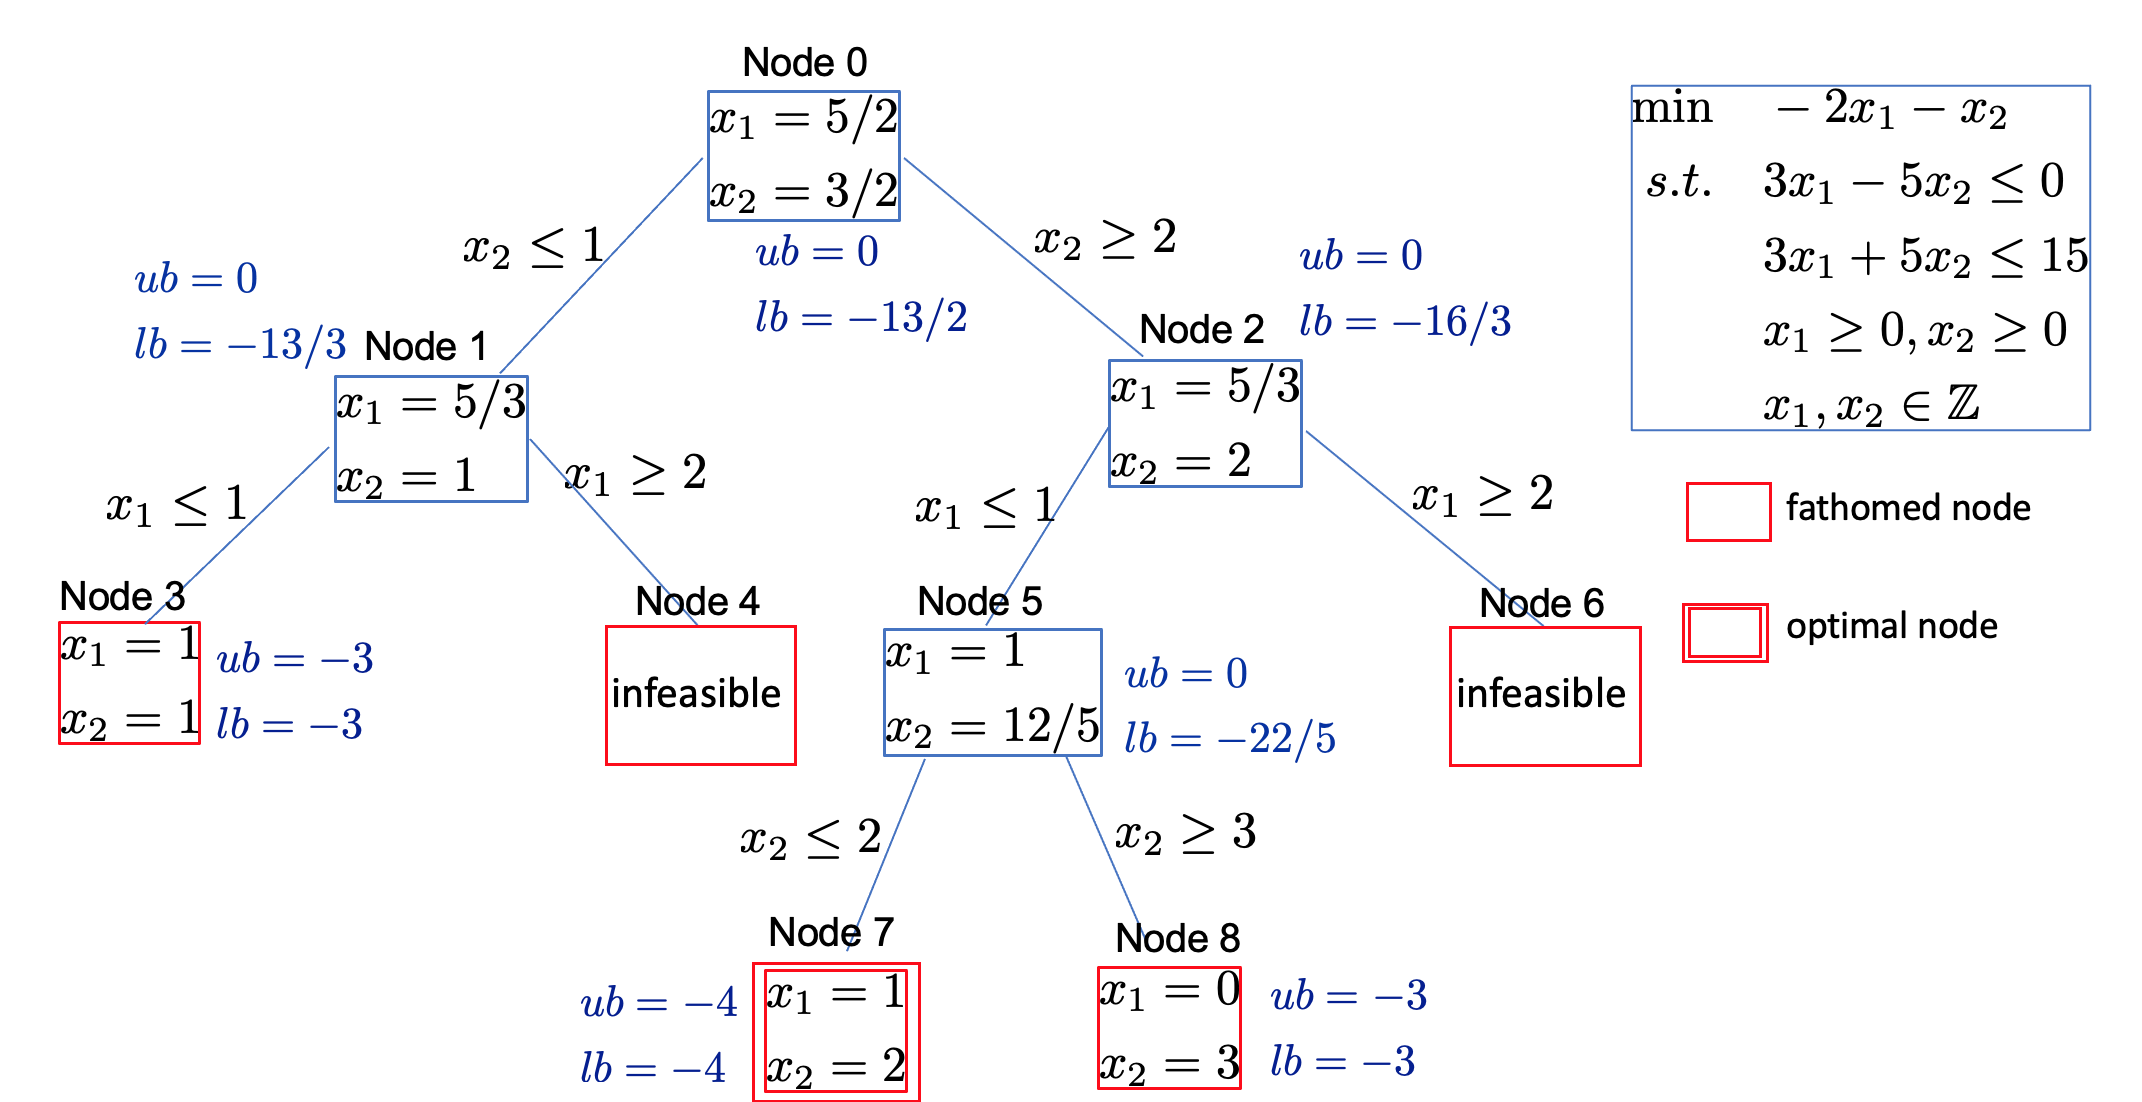
\includegraphics[width=0.75\textwidth]{./assets/advanced-programming/branch-and-bound.png}
	\caption{The Branch \& Bound algorithm on an example ILP.}
\end{figure}

\begin{algorithm}
	\caption{Branch \& bound}
	\label{alg:branch-and-bound}

	\SetKwProg{Fn}{Function}{:}{}
	\SetKwFunction{FBranchBound}{BranchAndBound}

	\Fn{\FBranchBound{$\max\{ \vec c^T \vec x \mid A \vec x \leq \vec b, \vec x \in \Z^n\}$,
			$\tilde{\vec x}$}}{
		$\vec x^* \gets \argmax\{ \vec c^T \vec x \mid A \vec x \leq \vec b\}$\;

		\If{LP relaxation is infeasible \textbf{or}
			$\vec c^T \vec x^* < \vec c^T \tilde{\vec x}$}{
			\Return Nothing\;
		}
		\ElseIf{$\vec x^* \in \Z^n$}{
			\Return $\vec x^*$\;
		}

		Choose $i \in \{1, \dots, n\}$ such that $x_i^* \notin \Z$\;
		$\tilde{\vec x} \gets $ \FBranchBound(
		$\max\{ \vec c^T \vec x \mid A \vec x \leq \vec b, x_i \leq \floor{x_i^*}, \vec x \in \Z^n\}$,
    $\tilde{\vec x}$
		) \;
		$\tilde{\vec x} \gets $ \FBranchBound(
		$\max\{ \vec c^T \vec x \mid A \vec x \leq \vec b, x_i \geq \floor{x_i^*}+1, \vec x \in \Z^n\}$,
    $\tilde{\vec x}$
		) \;

		\Return $\tilde{\vec x}$\;
	}
\end{algorithm}

Choosing which variable to branch on is kind of an open problem: there exists different heuristics
on it, some even try to us machine learning to find the best one.

\subsection{Total dual integrality}
\begin{definition}{Total dual integrality}{}
	A system $A\vec x \leq \vec b$ is TDI if its dual
	$\min\{\vec b^T \vec y\mid A^T \vec y = c, \vec y \geq 0 \}$ attains its minimum at an
	integer point $\vec y^*$ for any integer $\vec c$ such that the optimum exists and is finite.
\end{definition}

\begin{lemma}{}{}
	If $A$ is TU, then $A \vec x \leq \vec b$ is TDI for any integer $\vec b$.
\end{lemma}

\begin{theorem}{}{}
	If $A\vec x \leq \vec b$ is TDI, then $\{x \mid A \vec x \leq \vec b \}$ is an integer polyhedron.
\end{theorem}

\begin{proof}[Proof (sketch)]
	TODO: lec 22 thm 2
\end{proof}

\begin{theorem}{Giles-Pulleyblank}{}
	Any rational $P$ can be written as $P = \{ \vec x \mid A \vec x \leq \vec b \}$ such that $A$ is
	integer and $A \vec x \leq \vec b$ is TDI.

	Moreover, $P$ is integer if and only if $\vec b$ is integer.
\end{theorem}

\begin{proof}[Proof (idea)]
	For any minimal face $F$ of $P$ there exists some $\vec c$ so that $\vec c^T \vec x$ is maximized
	there.
	Indeed, there is a cone of such vectors $\vec c$: this cone is defined by the vectors
	perpendicular to the faces whose intersections form $F$.

	Consider the set of such vectors
	\begin{equation}
		K_F = \{ \vec c \mid \vec c^T \vec z = \max \{ \vec c^T \vec x \mid \vec x \in P\} \ \forall \vec z \in
		F \}
	\end{equation}
	and a set of vectors $\vec a_1, \dots, \vec a_t \in \Z^n_+$ such that
	every integer vector in $K_F$ is a non-negative combination of such vectors.
	This is called an Hilbert basis of $K_F$ and we can prove it always exists.

	Let $A^F$ be the matrix whose rows are the vectors $\vec a_1, \dots, \vec a_t$ and $\vec b^F$ be
	the vector where each entry is the solution of $\max \{\vec a^T_i \vec x \mid \vec \in P\}$ for
	$i \in \{1, \dots, t\}$.
	Then take $A$ be the concatenation of the rows of $A_F$ for all faces $F$ and the same for $\vec b$ and
	$\vec b^F$.
	In this way we are guaranteed to satisfy TDI.
\end{proof}

\subsection{Cutting planes}

Consider an halfspace $H = \{ \vec x \mid \vec c^T \vec x \leq \vec \delta \}$ and its integer hull
$H_I$, then $H_I \subseteq \{ \vec x \mid \vec c^T \vec x \leq \floor{\vec \delta} \}$.
Therefore we have found a way to \say{cut} some stuff without removing any integer point.

\begin{definition}{Gomory-Chvátal truncation}{gomory-chvatal}
	Let $P$ be a convex set.
	We define a truncation as
	\begin{equation}
		P' = \bigcup \{\vec x \mid \vec c^T \vec x \leq \floor{\vec \delta} \}
	\end{equation}
	where $\vec c$ is such that $P \subseteq \{ \vec x \mid \vec c^T \vec x \leq \vec \delta \}$.
\end{definition}

\begin{theorem}{Schrijver}{schrijver-1}
	Let $P = \{ \vec x \mid A \vec x \leq \vec b \}$ such that its system is TDI, $A$ is integer and
	$\vec b$ is rational.
	Then $P' = \{ \vec x \mid A\vec x \leq \floor{\vec b}\}$ is a valid truncation.
\end{theorem}

This is useful since we know we can always complete a polyhedron to a TDI system: after the first
truncation $P'$ may no longer be TDI, therefore we complete it again to be TDI, and truncate again,
and so on.

\begin{theorem}{Schrijver}{schrijver-2}
	For every rational polyhedron $P$ there exists $t \in \N_0$ finite such that the $t$-th truncation
	of $P$, $P^{(t)} = P_I$.

	We call $t$ the Chavátal rank of $P$.
\end{theorem}

\subsubsection{Gomory cuts}

We now look at how we can use this knowledge to speed up the execution of the branch and bound
algorithm. At each step of the algorithm we solve an LP relaxation, assume we are using the dual
simplex method.

We have reached an optimal tableau of the relaxation where there are some fractional variables, say
$x_i$ is fractional.

We now look at the $x_i$ row in the simplex tableau:
\begin{equation}
	x_i = p - k_1 x_{i_1} - \dots - k_e x_{i_\ell}
	- \alpha_1 x_{j_1} - \dots - \alpha_{\ell'} x_{j_{\ell'}}
\end{equation}
where we have ordered the coefficients so that $k_1, \dots, k_\ell \in \Z$ and
$\alpha_1, \dots, \alpha_{\ell'} \in \R$.
Then, since $\vec x$ is non-negative we can write
\begin{equation}
	x_i + k_1 x_{i_1} + \dots + k_e x_{i_\ell}
	+ \floor{\alpha_1} x_{j_1} + \dots + \floor{\alpha_{\ell'}} x_{j_{\ell'}} \leq p
\end{equation}
which is a valid inequality.
Then consider the truncation
\begin{equation}
	x_i + k_1 x_{i_1} + \dots + k_e x_{i_\ell}
	+ \floor{\alpha_1} x_{j_1} + \dots + \floor{\alpha_{\ell'}} x_{j_{\ell'}} \leq \floor{p}
\end{equation}
and we add it as constraint to the original LP and we continue iterating.

\section{Convex optimization}

\subsection{Introduction}

\begin{definition}{Convex function}{convex-fn}
	Let $\mathcal D \subseteq \R^d$ convex and $f: \mathcal D \to \R$.
	Then $f$ is convex if for all $x, y \in \mathcal D$ and $\alpha \in [0, 1]$ we have
	\begin{equation}
		f(\alpha x + \overline{\alpha} y) \leq \alpha f(x) + \overline \alpha f(y)
	\end{equation}
	where $\overline \alpha = (1-\alpha)$.
\end{definition}

As we know that a differentiable $f$ is convex if and only if its domain is convex and
\begin{equation}
	f(y) \geq f(x) + \grad f(x)^T(y-x)
\end{equation}
that is, its first order approximation is smaller than the value itself.
This is quite useful because it tells us that if $\grad f(x) = 0$ we have found a local minimum.


\begin{definition}{Convex program}{convex-program}
	Let $\mathcal D \subseteq \R^n$ convex and $f_0, f_1, \dots, f_m, h_1, \dots, h_p: \mathcal D \to \R$
	be convex functions.
	The following minimization problem is a convex program in standard form:
	\begin{align}
		\min f_0(x)         &                              \\
		\text{s.t. }	f_i(x) & \leq 0 \quad i = 1, \dots, m \\
		h_i(x)              & = 0    \quad i = 1, \dots, p
	\end{align}
\end{definition}

\begin{definition}{Lagrangian}{lagrangian}
	A function $L: (\mathcal D \cross \R^m \cross \R^p) \to \R$ is the lagrangian of a convex
	program if
	\begin{equation}
		L(x, \lambda, \nu) = f_0(x) + \sum_{i = 1}^m \lambda_i f_i(x) + \sum_{i = 1}^p \nu_i h_i(x)
	\end{equation}
	where $\lambda_i, \nu_i$ are called \emph{lagrangian multipliers}, while
	the vectors $\vec \lambda, \vec \nu$ are called \emph{dual variables}.
\end{definition}

Using the lagrangian we can express the primal as
\begin{equation}
	p^* = \inf_{x \in \mathcal D} \sup_{\substack{\lambda \geq 0 \\ \nu}} L(x, \lambda, \nu)
\end{equation}
and the dual as
\begin{equation}
	q^* = \sup_{\substack{\lambda \geq 0 \\ \nu}} \inf_{x \in \mathcal D} L(x, \lambda, \nu)
\end{equation}

\begin{definition}{Lagrangian dual}{lagrangian-dual}
	The lagrangian dual problem (or just dual) of a convex optimization problem is defined as
	\begin{align}
		\max_{\lambda, \nu} \left(\inf_{x\in \mathcal D} L(x, \lambda, \nu) \right) &        \\
		\text{s.t. }	\lambda                                                        & \geq 0
	\end{align}
	where $L$ is the lagrangian of the primal as defined in \cref{def:lagrangian}.
\end{definition}

TODO: weak duality holds, see lecture 7.

However strong duality does not: in fact we can construct a counter example where
the optimal solutions exist and do not coincide.
Consider the following program over the domain $\mathcal D = \{(x, y) \mid y \geq 0 \}$
\begin{align}
	\min e^{-x} & \\
	\text{s.t. }	\frac{x^2}{y} \leq 0
\end{align}
We have that the optimal objective value is $e^0 = 1 = p^*$ with $x^* = 0$.
The lagrangian is $L(x, y, \lambda) = e^{-x} + \lambda \frac{x^2}{y}$
and the dual function is $g(\lambda) = \inf_{x, y \gt 0} (e^{-x} + \lambda x^2/y)$
which is $0$ if $\lambda \geq 0$ and $-\infty$ if $\lambda < 0$.
Then the solution to the dual is $\max_{\lambda \geq 0} g(\lambda) = 0 = d^*$
and $p^* \neq d^*$.

We want to find another condition to add to the strong duality theorem for it to hold
even in convex programs.

\subsubsection{Slater's constraints}

\begin{theorem}{Slater's theorem}{slaters}
	Consider the following convex program
	\begin{align}
		\min f_0(x)         &                              \\
		\text{s.t. }	f_i(x) & \leq 0 \quad i = 1, \dots, m \\
		A x                 & = b
	\end{align}
	such that $x \in \mathrm{int}(\mathcal D)$ and $f_i \lt 0$ for all $i = 1, \dots, m$ where
	$f_i$ is not affine.
	Note that all the $h_i$ are affine and can therefore be summarized as a matrix.

	Then strong duality holds (cf. \cref{thm:strong-duality}).
\end{theorem}

Note that these conditions these are not the only conditions for strong duality to hold, we will
discuss more in the future.
Moreover, Slanter's conditions ensure that an optimal solution exists.
These conditions are automatically satisfied by linear programs.

\begin{proof}
	Consider the following sets:
	\begin{align}
		\mathcal G & = \{ (f_0(x), f_1(x), \dots, f_m(x), h_1(x), \dots, h_p(x)) \mid x \in \mathcal D\} \\
		\mathcal A & = \left\{ (u, v, t) \mid \exists x \in \mathcal D \text{ s.t. }
		\substack{f_i(x) \leq u_i \enspace \forall i = 1, \dots, m                                       \\
		h_i(x) = v_i \enspace \forall i = 1, \dots, p                                                    \\
			f_0(x) \leq t
		} \right\}
	\end{align}

	Then we can write the optimal solution for the primal equivalently as
	\begin{align}
		p^* & = \inf \{ t \mid (u, v, t) \in \mathcal G, u \leq 0, v = 0\} \\
		    & = \inf \{ t \mid (0, 0, t) \in \mathcal A\}
	\end{align}
	We can also write the dual function as
	\begin{align}
		g(\lambda, \nu) & = \inf \{(\lambda, \nu, 1)^T(u, v, t) \mid (u, v, t) \in \mathcal G \} \\
		                & = \inf \{(\lambda, \nu, 1)^T(u, v, t) \mid (u, v, t) \in \mathcal A \}
	\end{align}
	where we notice that $(\lambda, \nu, 1)^T(u, v, t)$ is the lagrangian.

	The next step is to prove that $\mathcal A$ is convex.
	To do so we consider $(u, v, t) = x, (u', v', t') = x' \in \mathcal A$
	and $\tau \in [0, 1]$.
	We want to show that $\overline x = \tau (u, v, t) + \overline \tau(u', v', t') \in \mathcal A$.
	\begin{align}
		f_0(\overline x) & \leq \tau t + \overline \tau t     & \text{by convexity of } f_0 \\
		f_i(\overline x) & \leq \tau u_i + \overline \tau u_i & \text{by convexity of } f_i \\
		h_i(\overline x) & \leq \tau v_i + \overline \tau v_i & \text{by affinity of } h_i
	\end{align}
	therefore $\overline x \in \mathcal A$.

	Now we are ready to prove the actual theorem.
	We assume $\rank(A) = p$ (otherwise we remove the redundant constraints).
	If $p^* = -\infty$ by weak duality also $d^* = -\infty$, hence we just need to consider the cases
	where $p^*$ is finite.
	Let us define another set
	\begin{equation}
		\mathcal B = \{(0,0,s) \in \R^m \cross \R^n \cross \R \mid s < p^* \}
	\end{equation}
	then $\mathcal A \cap \mathcal B = \varnothing$ since otherwise it would imply that
	there exists a feasible $x \in \mathcal D$ and $f_0(x) = t < p^*$ which contradicts the fact that
	$p^*$ is optimal.

	Since they are both convex we use \cref{thm:weak-conv-sep} to find a hyperplane
	$h = \{(u, v, t) \mid (\overline \lambda, \overline \nu, \mu)^T (u, v, t) = \alpha \}$
	such that
	\begin{align}
		\overline \lambda^T u + \overline \nu^T v + \mu t & \geq \alpha \quad \forall (u, v, t) \in \mathcal A \\
		\overline \lambda^T u + \overline \nu^T v + \mu t & \leq \alpha \quad \forall (u, v, t) \in \mathcal B
	\end{align}
	then for every $x \in \mathcal D$ we have
	\begin{equation}
		\sum_{i = 1}^m \lambda_i f_i(x) + \overline \nu^T(Ax - b) + \mu f_0(x) \geq \alpha \geq \overline \mu p^*
		\label{eq:weird-lagrangian}
	\end{equation}
	which is very similar to the lagrangian with an extra $\mu$ term.

	Now we consider two cases based on $\mu$:
	\begin{enumerate}[label=\roman*.]
		\item $\mu > 0$. We divide everything by $\mu$ to get the lagrangian
		      \begin{equation}
			      L(x, \lambda, \nu) =
			      L\left( x, \frac{\overline \lambda}{\mu}, \frac{\overline \nu}{\mu} \right)
			      \geq p^*
		      \end{equation}
		      which means $g(\lambda, \nu) \geq p^*$ and since $g(\lambda, \nu)\leq p^*$ already holds
		      by weal duality we conclude that $g(\lambda, \nu) = p^*$ and $(\lambda, \nu)$ is the
		      optimal solution to the dual.
		\item $\mu = 0$.
		      The idea is that we have that
		      $h = \{(u, v, t) \mid (\overline \lambda, \overline \nu, 0)^T (u, v, t) = \alpha \}$
		      which means that the plane is vertical since it does not depend on $t$.

		      If we substitute $\mu = 0$ in \cref{eq:weird-lagrangian} we get
		      \begin{equation}
			      \sum_{i = 1}^m \lambda_i f_i(x) + \overline \nu^T(Ax - b)  \geq 0
		      \end{equation}
		      Now we apply feasibility, that is $Ax - b = 0$, to get
		      \begin{equation}
			      \sum_{i = 1}^m \lambda_i f_i(x) \geq 0
		      \end{equation}
		      but by Slater's conditions we have that $f_i(\overline x) < 0$,
		      therefore $\overline \lambda = 0$.

		      Then our hyperplane, which is defined by $(\overline \lambda, \overline \nu, \mu)$, needs
		      to be $\neq 0$, since $0$ does not define an hyperplane: necessarily we have that
		      $\overline \nu \neq 0$.

		      From before we know that $\overline \nu^T (Ax - b) = 0$ which fives us two cases:
		      \begin{itemize}
			      \item If $\overline \nu^T A \neq 0$ then there exists $x \in \mathcal D$ such that
			            $\overline \nu^T(Ax - b) < 0$;
			      \item If $\overline \nu^T A = 0$ then $A$ has some linearly dependent rows.
		      \end{itemize}
		      In both cases we have reached a contradiction, therefore $\mu$ cannot be $0$.
		      \qedhere
	\end{enumerate}
\end{proof}

\begin{example}{Least squares}{least-squares}
	Write the dual of the following convex problem:
	\begin{align}
		\min x^T x       &     \\
		\text{s.t. }	A x & = b
	\end{align}
\end{example}

\begin{proof}[Solution]
	The lagrangian is
	\begin{equation}
		L(x, \nu) = x^T x + \nu^T (Ax - b)
	\end{equation}
	(notice we do not have $\lambda$.)
	Now we want to minimize the lagrangian w.r.t. $x$: since it is differentiable we can solve
	$\grad_x L(x, \nu) = 0$, that is
	\begin{equation}
		2x + A^T \nu = 0 \implies x = - \frac{A^T \nu}{2}
	\end{equation}
	then the dual can be written as
	\begin{equation}
		\max_{\nu} \left(-\frac{1}{4}\right) \nu^T A A^T \nu - b^T \nu
	\end{equation}
\end{proof}

\subsubsection{KKT Conditions}
In linear programming we had some ways to check whether a solution was optimal.
In convex programming we have something similar.

\begin{theorem}{KKT}{kkt-cond}
	Consider a convex problem as in \cref{def:convex-program} where $f_0, f_1, \dots, f_m, h_1, \dots, h_p$
	are differentiable.
	Let $x^*$ be a solution to the primal and $(\lambda^*, \nu^*)$ a solution to the dual.
	Then $x^*$ and $(\lambda^*, \nu^*)$ are optimal and $d^* = p^*$ if and only if all the following
	conditions are true:
	\begin{enumerate}[label=(\roman*.)]
		\item $f_i(x^*) \leq 0 \enspace \forall i = 1, \dots, m$
		\item $h_i(x^*) = 0 \enspace \forall i = 1, \dots, p$
		\item $\lambda_i^* \geq 0 \enspace \forall i = 1, \dots, m$
		\item $\lambda^*_i f_i(x^*) = 0 \enspace \forall i = 1, \dots, m$
		\item $\grad f_0(x^*) + \sum \lambda_i^* \grad f_i(x^*) + \sum \nu_i^* \grad h_i(x^*) = 0$
	\end{enumerate}
\end{theorem}

\begin{proof}
	We prove each implication separately.
	\begin{description}
		\item[Optimality implies KKT conditions]
		      Conditions (i.), (ii.), and (iii.) are true since they are implied
		      by the feasibility of the primal and the dual.

		      To show (iv.) and (v.) we use the fact that we have optimal solutions:
		      \begin{align}
			      f_0(x^*) & = g(\lambda^*, \nu^*)                                                                                            \\
			               & = \inf_{x} f_0(x) + \sum \lambda_i^* f_i(x) + \sum \nu_i^* h_i(x)                                                \\
			               & \cancelto{=}{\leq} f_0(x^*) + \cancelto{\leq 0}{\sum \lambda_i^* f_i(x^*)} + \cancelto{0}{\sum \nu_i^* h_i(x^*)} \\
			               & \cancelto{=}{\leq} f_0(x^*)
		      \end{align}
		      where we put $=$ instead of $\leq$ since $x^*$ is minimizer of the lagrangian and
		      the last equality holds because (by feasibility) we have that $\lambda_i^* \geq 0$
		      and $f_i(x^*) \leq 0$.
		      This proves (v.) and (iv.) comes from the fact that $\sum \lambda_i^* f_i(x^*) = 0$
		      and every term is non-positive.
		\item[KKT conditions imply optimality]
		      Conditions (i.), (ii.) and (iii.) imply feasibility of the primal and the dual.

		      Since $\lambda_i \geq 0$, $L$ is the sum of convex functions so it is also convex.
		      Moreover, we use (v.), which tells us that $x^*$ is a minimizer, to write
		      \begin{align}
			      g(\lambda^*, \nu^*) & = L(x^*, \lambda^*, \nu^*)                                                                   \\
			                          & = f_0(x^*) + \cancelto{= 0}{\sum \lambda_i^* f_i(x^*)} + \cancelto{0}{\sum \nu_i^* h_i(x^*)} \\
			                          & = f_0(x^*)
		      \end{align}
		      where we cancelled the first term using (iv.) and the second one by feasibility.
		      \qedhere
	\end{description}
\end{proof}

\subsection{Equivalent characterizations of convexity}

TODO: lec 25

\subsection{Gradient descent}

TODO: lec 25

\subsubsection{Vanilla analysis}

TODO: lec 25

\subsubsection{Smooth convex functions}

\begin{definition}{$L$-smooth convex function}{smooth-convex-function}
	A function $f$ is smooth convex if $f$ is convex and
	\begin{equation}
		f(y) \leq f(x) + \grad f(x)^T (y-x) + \frac{L}{2} \norm{ x - y}^2
	\end{equation}
	for all $x, y \in X$, where $L$ is a constant.
\end{definition}

Note that this definition is different from the one given in the analysis courses and it has a
different meaning.

Notably, if $L = 0$, we have that $f(y) = \grad f(x)^T (y - x)$ for all $x, y \in X$ and $f$ is
affine. This is because we have \say{$\leq$} because of convexity and \say{$\geq$} because of
$0$-smoothness.

Consider $f(x) = x^2$. We have that this function is $2$-smooth.
Indeed we have
\begin{equation}
	f(y) = f(x) + 2x(y - x) + (x+y)^2 = f(x) + f'(x)(y-x) + \frac{L}{2} (x-y)^2
\end{equation}

If instead we have a quadratic function defined by a matrix such as
\begin{equation}
	f(x) = x^T Q x + b^T x + c \quad \text{with } Q \in \R^{d\cross d}, b \in \R^d, c\in \R
\end{equation}
we will be able to say that $f(x)$ is $2 \norm{Q}$-smooth (where $\norm{Q}$ is the spectral norm).

A function like $f(x) = x^4$ instead is not smooth, since it grows faster than the quadratic
approximation.

\begin{lemma}{Observations about $L$-smooth functions}{}
	\begin{itemize}
		\item Only functions whose growth is quadratic can be smooth.
		\item A function $f: \R^d \to \R$ which is convex and differentiable is $L$-smooth if and only
		      if $\grad f$ is $L$-Lipschitz.
		\item Let $f_i$ be $L_i$ smooth, and $\lambda_i \in \R^+$ for $i \in \{1, \dots, m\}$.
		      Then $f = \sum_{i = 1}^{m} \lambda_i f_i$ is $(\sum_{i = 1}^{m} \lambda_i L_i)$-smooth over the
		      intersection of the domains.
		\item Let $f: X \subseteq \R^d \to \R$ be $L$-smooth and $g(x) = Ax + b$ for
		      $A \in \R^{d \cross m}$ and $b \in \R^d$.
		      Then $f \circ g$ is $L\norm{A}^2$-smooth where the composition exists.
	\end{itemize}
\end{lemma}

\begin{proposition}{Gradient descent for smooth functions (step)}{gradient-descent-for-smooth-functions}
	Let $f: \R^d \to \R$ be $L$-smooth and let $\gamma$ be the step size defined as
	$\gamma = \frac{1}{L}$.
	Then GD satisfies
	\begin{equation}
		f(x_{t+1}) \leq f(x_t) - \frac{1}{2L} \norm{\grad f(x_t)}^2
	\end{equation}

	In particular, it is enough to require $f$ to be $L$-smooth on the segment joining $f(x_{t+1})$ to
	$f(x_t)$.
\end{proposition}

Note that this means that $f(x_{t+1}) \leq f(x_t)$ for every $t$, which was something we didn't have
in the case for Lipschitz functions.

\begin{proof}
	TODO: lec 26, lemma 5
\end{proof}

\begin{theorem}{Gradient descent for smooth functions}{gradient-descent-for-smooth-functions}
	Let $f: \R^d \to \R$ be $L$-smooth and let $\gamma$ be the step size defined as
	$\gamma = \frac{1}{L}$.
	Then GD achieves at iteration $T$
	\begin{equation}
		f(x_T) - f(x^*) \leq \frac{L}{2T} \norm{x_0 - x^*}^2
	\end{equation}
	where $x^*$ is the global minimum of $f$.
\end{theorem}
\begin{proof}
	TODO: lec 26, thm 6
\end{proof}

\begin{corollary}{Convergence rate for GD of $L$-smooth functions}{convergence-rate-for-gd-of-l-smooth-functions}
	If we want $f(x_T) - f(x^*) < \varepsilon$ we need $T \geq \frac{R^2 L}{2 \varepsilon}$ where
	$R = \norm{x_0 - x^*}^2$.
\end{corollary}

\begin{proof}
	Just sum the gradient descent equation over each step, this will give a telescopic sum:
	\begin{equation}
		\frac{1}{2L} \sum_{T-1}^{t=0} \norm{\grad f(x_t)}^2 \leq f(x_0) - f(x_t)
	\end{equation}

	By what we did in vanilla analysis we get
	\begin{align}
		\sum_{T-1}^{t=0} \norm{\grad f(x_t)}^2 & \leq \sum_{T-1}^{t = 0} \norm{g_t}^2 + \frac{L}{2} \norm{x_0 - x^*}^2 \\
		                                       & \leq f(x_0) - f(x_T) + \frac{L}{2} \norm{x_0 - x^*}^2                 \\
	\end{align}
	Now we will move $f(x_0)$ and $f(x_T)$ on the left, so that $f(x_0)$ is cancelled and we get
	\begin{equation}
		\frac{1}{2L} \sum_{T}^{t=1} \norm{\grad f(x_t)}^2 \leq \frac{L}{2} \norm{x_0 - x^*}^2
	\end{equation}

	Now using the fact that $f(x_T) - f(x_t) \geq 0$ for all $t$ we get
	\begin{equation}
		f(x_T) - f(x^*) \leq \frac{1}{T} \sum_{T}^{t = 1} (f(x_t) - f(x^*)) \leq
		\frac{L}{2T} \norm{x_0 - x^*}^2
	\end{equation}
	and we obtain a bound on the average error.
\end{proof}

\subsubsection{Strong convexity}

\begin{definition}{Strong convexity}{strong-convexity}
	Let $f$ be convex and differential. Let $X \subseteq \dom(f)$ convex and a parameter
	$\mu > 0$.
	We say that $f$ is $\mu$-strongly convex over $X$ if
	\begin{equation}
		f(y) \leq f(x) + \grad f(x)^T (y - x) + \frac{\mu}{2} \norm{x-y}^2
	\end{equation}
	for all $x \in X$.
\end{definition}

While smoothness told us that the growth needs to be at most quadratic, strong convexity tells us
that the growth should be at least quadratic.

\begin{proposition}{Global minimum in strong convexity}{global-minimum-in-strong-convexity}
	A $\mu$-strong convex function as an unique global minimum $x^*$.
\end{proposition}

\begin{proof}
	First we claim that if a minimizer $x^*$ exists then it is unique.
	For $x^*$ to be a minimizer we need $\grad f(x^*) = 0$, therefore for all $y \in X$ we have
	\begin{equation}
		f(y) \geq f(x^*) + \frac{\mu}{2} \norm{x^* - y}^2 > f(x^*)
	\end{equation}
	unless $x^* = y$ since $\mu > 0$.

	Then we claim that $x^*$ exists.
	Let $x_0 \in \R^d$. Then there exists $R > 0$ so that $f(y) > f(x_0)$ if
	$\norm{x_0 - y} > R$. This is because, if $R$ is large enough, the quadratic term (which is always
	positive) will dominate the linear term (which could also be negative).
	Then we consider the closed ball $B_R(x_0)$ where we know that $f$ will attain a minimum
	(Weierstrass) which we will call $x^*$. We have that $f(x^*)$ is less than any $f(x)$ with
	$x \notin B_R(x_0)$ since $f(x_0) < f(x)$.
\end{proof}

TODO: lec 27

\subsubsection{Projection gradient descent}

TODO: lec 27

\subsubsection{Subgradient descent}

Sometimes we will have to work with non-differentiable functions: even if we are not able to compute
the gradient we can use a surrogate.

\begin{definition}{Subgradient}{subgradient}
	Let $f: \dom(f) \subseteq \R^d \to \R$. Then $g \in \R^d$ is a subgradient of $f$ at
	$x \in \dom(f)$ if
	\begin{equation}
		f(y) \geq f(x) + g^T(y - x) \quad \forall g \in \dom(f)
	\end{equation}

	We denote $\partial f(x)$ the set of subgradients of $f$ at point $x$.
\end{definition}

\begin{remark}{}{}
	If $f$ is differentiable at $x \in \dom(f)$, then
	$\partial f(x) \subseteq \{ \grad f(x) \}$.
\end{remark}

\begin{remark}{}{}
	\begin{equation}
		f: \dom(f) \to \R \text{ is convex } \iff \dom(f) \text{ is convex and }
		\partial f(x) \neq \varnothing \enspace \forall x \in \mathrm{int. dom}(f)
	\end{equation}
\end{remark}

\begin{remark}{}{}
	Let $f: \dom (f) \to \R^d$ is convex, $\dom(f)$ is open and $B \in \R_+$.
	Then
	\begin{equation}
		\norm{g} \leq B \enspace \forall x \in \dom(f), g \in \partial f(x) \iff \abs{f(x) - f(y)} \leq
		B \norm{x-y}
	\end{equation}
\end{remark}

\begin{remark}{}{}
	If $0 \in \partial f(x)$, then $x$ is a global minimizer of $f$.
\end{remark}

\begin{proof}
	\begin{equation}
		f(y) \geq f(x) + 0^T (y-x) = f(x)
	\end{equation}
\end{proof}

\begin{remark}{}{}
	If $f: \dom (f) \to \R^d$ is convex and $\dom(f) \subseteq \R^d$ is open, for $x \in \dom(f)$ we
	have
	\begin{equation}
		\partial f(x) =
		\conv \left( \{ \lim_{n \to \infty} \grad f(x_n) \mid \lim_{n \to \infty} x_n = x \} \right)
	\end{equation}
\end{remark}

\begin{theorem}{Subgradient descent}{subgradient-descent}
	Choose any $g_t \in \partial f(x_t)$ and define $x_{t+1} = x_t - \gamma_t g_t$. Then, in the same
	setting as TODO: Lipschitz gradient descent, we obtain the same error bound.
\end{theorem}

\begin{proof}
	This is exactly the same proof, we just substitute the gradient with the subgradient.
\end{proof}

We will not consider the case of smooth functions as this doesn't make sense in the case of non
differentiable functions.

\begin{definition}{Strong convexity for non-differentiable functions}{strong-convexity-for-non-differentiable-functions}
	Let $f: \dom(f) \to \R$ convex and $\mu > 0$.
	$f$ is $\mu$-strongly convex if
	\begin{equation}
		f(y) \geq f(x) + g^T(y- x) + \frac{\mu}{2} \norm{y - x}^2 \quad \forall x, y \in \dom (f),
		\forall g \in \partial f(x)
	\end{equation}
\end{definition}

\begin{theorem}{Subgradient descent for strong convex functions}{subgradient-descent-for-strong-convex-functions}
	Let $f: \R^d \to \R$ be $\mu$-strongly convex and $x^*$ the global minimum of $f$.
	Let $\gamma_t = \frac{2}{\mu(t+1)}$, then
	\begin{equation}
		f\left( \frac{2}{T(T+1)} \sum_{}^{} t x_t \right) - f(x^*) \leq \frac{2 B^2}{\mu(T+1)}
	\end{equation}
	where $B = \max_{t} \norm{g_t}$.
\end{theorem}
\begin{proof}
	Start with vanilla analysis:
	\begin{equation}
		g_t^T(x_t - x^*) = \frac{\gamma_t}{t} \norm{g_t}^2 + \frac{1}{2 \gamma_t} ( \norm{x_t - x^*}^2 -
		\norm{x_{t+1} - x^*}^2)
	\end{equation}
	and apply strong convexity. We get
	\begin{equation}
		f(x_t) - f(x^*) \leq \frac{\gamma_t}{2} B^2 + \frac{\gamma_t^{-1} - \mu}{2} \norm{x_t - x^*}^2 -
		\frac{\gamma_t^{-1}}{2} \norm{x_{t+1} - x^*}^2
	\end{equation}

	We now want to sum over all the iterations and obtain a telescopic sum. However we have different
	coefficients on the second part, therefore we have to do a little more work.

	In order for the sum to telescope we need to impose
	\begin{equation}
		\frac{\gamma^{-1}_{t+1} - \mu}{2} = \frac{\gamma_t^{-1}}{2} \implies
		\gamma_{t}^{-1} = \mu(t+1)
	\end{equation}

	We get
	\begin{equation}
		\sum_{t = 1}^{T} \left( f(x_t) - f(x^*) \right) \leq \frac{B^2}{2} \sum_{t = 1}^{T} \gamma_t +
		\frac{\mu}{2} \sum_{t = 1}^{T} \left( t \norm{x_t - x^*}^2 - (t-1) \norm{x_{t+1} - x^*}^2
		\right)
	\end{equation}
	then we divide by $T$ and obtain
	\begin{equation}
		\frac{1}{T} \sum_{t = 1}^{T} \left( f(x_t) - f(x^*) \right) \leq \frac{B^2}{2T} \sum_{t = 1}^{T}
		\gamma_t + \frac{\mu}{2} \left( \norm{x_t - x^*}^2 \right)
	\end{equation}
	where the sum over $\gamma_t$ gives us
	\begin{equation}
		\frac{1}{\mu} \sum_{t = 1}^{T} \frac{1}{t + 1} = \frac{1}{\mu} O(\log T)
	\end{equation}
	from some analysis trickery.

	We therefore get a bound of $\O\left(\frac{\log T}{T} \right)$.

	But this is not the best bound, if instead we choose $\gamma$ as in the theorem statement we get
	\begin{equation}
		f(x_t) - f(x^*) \leq \frac{B^2}{\mu(t+1)} + \frac{\mu}{4} \left((t-1) \norm{x_t - x^*}^2 -
		(t+1) \norm{x_{t+1} - x^*}^2\right)
	\end{equation}
	and to make the sum telescope we multiply both sides by $t$
	\begin{equation}
		t\left(f(x_t) - f(x^*)\right) \leq \frac{B^2 t}{\mu(t+1)} + \frac{\mu}{4}
		\left(t(t-1) \norm{x_t - x^*}^2 - t(t+1) \norm{x_{t+1} - x^*}^2\right)
	\end{equation}

	We can now expand the sum to get
	\begin{equation}
		\sum_{t = 1}^{T} t\left(f(x_t) - f(x^*)\right) \leq \frac{T B^2}{\mu(t+1)} -
		\frac{\mu}{4} \left( T(T+1) \norm{x_{t+1} - x^*}^2\right) \leq \frac{TB^2}{\mu}
	\end{equation}

	Then, by Jensen inequality, we get
	\begin{equation}
		f\left(\frac{2}{T(T+1)} \sum_{t = 1}^{T} x_t\right) - f(x^*) \leq
		\frac{2}{T(T+1)} \sum_{t = 1}^{T} t(f( x_t) - f(x^*)) \leq \frac{2B^2}{\mu(T+1)}
	\end{equation}

	Note that $R$ does not appear in this result. This is because our function is strongly convex,
	therefore the further away we start, the larger $B$ will be; hence $R$ is somehow implicit in $B$.
\end{proof}

\begin{theorem}{Nesterov}{nesterov}
	For all $T \leq d-1$ and starting point $x_0$, $\exists f$ $B$-Lipschitz over $\R^d$ such that any
	(sub)-gradient method has an error
	\begin{equation}
		f(x_T) - f(x^*) \geq \frac{RB}{2(1+\sqrt{T + 1})}
	\end{equation}
\end{theorem}


\begin{theorem}{Nesterovski-Yudin}{nesterovski-yudin}
	For all $T \leq d-1$ and starting point $x_0$, $\exists f$ $L$-smooth over $\R^d$ such that any
	(sub)-gradient method has an error
	\begin{equation}
		f(x_T) - f(x^*) \geq \frac{3L \norm{x_0 - x^*}^2}{32 T^2}
	\end{equation}
\end{theorem}

\subsubsection{Accelerated gradient descent}

Start with $z_0 = y_0 = x_0$,
take $y_{t+1} = x_t - \frac{1}{L} \grad f(x_t)$,
$z_{t+1} = z_t - \frac{t+1}{2L} \grad f(x_t)$ and
$x_{t+1} = \frac{t+1}{t+3} y_{t+1} + \frac{2}{t+3} z_{t+1}$.

This algorithms has convergence rate of $\O\left(\frac{1}{T^2}\right)$ but nobody knows why.

\end{document}
